\documentclass [11pt,twoside]{article}
\usepackage[utf8]{inputenc}
\usepackage[T1]{fontenc}

%Page margins, header and footer positions
\usepackage{geometry}
 \geometry{
 a4paper,
 total={210mm,297mm},
 left=25mm,
 right=25mm,
 top=30mm,
 bottom=25mm,
 headsep=7mm}

\interfootnotelinepenalty=10000

%To display filling dots in the TOC for all entries
\usepackage[titles]{tocloft}
\renewcommand{\cftsecleader}{\cftdotfill{\cftdotsep}}

%Define new header and footer style
\usepackage{fancyhdr}

\pagestyle{fancy}
\fancyhf{}
\lhead{\color{Gray}{\small{Travlendar+ project by Andrea Mafessoni, Andrea Mazzeo, Daniele Moltisanti}}}
\lfoot{\textcolor{Gray}{\small{Copyright © 2017, Andrea Mafessoni, Andrea Mazzeo, Daniele Moltisanti – All rights reserved}}}
\rfoot{\textcolor{Gray}{\thepage}}
\renewcommand{\headrulewidth}{0pt}

%PACKAGES
\usepackage{wasysym}
\usepackage{pifont}

\newcommand{\supported}{\ding{52}\xspace}
\newcommand{\unsupported}{\ding{55}\xspace}
\newcommand{\partsupported}{\textcolor{black!40}{\ding{52}}\xspace}
\newcommand{\lowsupported}{\textcolor{black!20}{\ding{52}}\xspace}
\newcommand{\unknowsupported}{\textbf{?}\xspace}

%Font: Times
\usepackage{times}
%Change monospaced font
\renewcommand{\ttdefault}{lmtt}

%tables
\usepackage{tabu}
\usepackage{tabularx}
\usepackage{ltablex}
\usepackage{longtable}
\usepackage{float} % To allow the use of H modifier in long tables

%landscape mode
\usepackage{pdflscape}
\usepackage{rotating}
\usepackage{caption}

%make landscape mode be sensitive to even and odd pages
%start
\def\myrotate{\ifodd\c@page\else-\fi 90}
\makeatletter
\global\let\orig@begin@landscape=\landscape%
\global\let\orig@end@landscape=\endlandscape%
\gdef\@true{1}
\gdef\@false{0}
\gdef\landscape{%
    \global\let\within@landscape=\@true%
    \orig@begin@landscape%
}%
\gdef\endlandscape{%
    \orig@end@landscape%
    \global\let\within@landscape=\@false%
}%
\@ifpackageloaded{pdflscape}{%
    \gdef\pdf@landscape@rotate{\PLS@Rotate}%
}{
    \gdef\pdf@landscape@rotate#1{}%
}
\let\latex@outputpage\@outputpage
\def\@outputpage{
    \ifx\within@landscape\@true%
        \if@twoside%
            \ifodd\c@page%
                \gdef\LS@rot{\setbox\@outputbox\vbox{%
                    \pdf@landscape@rotate{-90}%
                    \hbox{\rotatebox{90}{\hbox{\rotatebox{180}{\box\@outputbox}}}}}%
                }%
            \else%
                \gdef\LS@rot{\setbox\@outputbox\vbox{%
                    \pdf@landscape@rotate{+90}%
                    \hbox{\rotatebox{90}{\hbox{\rotatebox{0}{\box\@outputbox}}}}}%
                }%
            \fi%
        \else%
            \gdef\LS@rot{\setbox\@outputbox\vbox{%
                \pdf@landscape@rotate{+90}%
                \hbox{\rotatebox{90}{\hbox{\rotatebox{0}{\box\@outputbox}}}}}%
            }%
        \fi%
    \fi%
    \latex@outputpage%
}
\makeatother
%end

%graphics
\usepackage{graphicx}
\usepackage[dvipsnames, table]{xcolor}
%If you upload images from PC, you need to insert code for the path here (different for Windows and Unix OS)

%References
%\usepackage{xpatch}
%\usepackage[backend=biber, style=numeric, citestyle=numeric, sorting=none]{biblatex}
%\addbibresource{main.bib}

%Other
\usepackage{ifthen}
\usepackage{xspace}
\usepackage{enumitem}
\usepackage{amssymb}
\usepackage[pdftex, colorlinks]{hyperref}
\newcommand{\comment}[1]{{\color{Red}$\blacktriangleright$ Comment: #1 $\blacktriangleleft$}}


% Some utilities\ldots
\usepackage{soul}
\usepackage{tikz}

\usetikzlibrary{calc}
\usetikzlibrary{decorations.pathmorphing}


\makeatletter

\newcommand{\defhighlighter}[3][]{%
  \tikzset{every highlighter/.style={color=#2, fill opacity=#3, #1}}%
}

\defhighlighter{yellow}{.5}

\newcommand{\highlight@DoHighlight}{
  \fill [ decoration = {random steps, amplitude=1pt, segment length=15pt}
        , outer sep = -15pt, inner sep = 0pt, decorate
       , every highlighter, this highlighter ]
        ($(begin highlight)+(0,8pt)$) rectangle ($(end highlight)+(0,-3pt)$) ;
}

\newcommand{\highlight@BeginHighlight}{
  \coordinate (begin highlight) at (0,0) ;
}

\newcommand{\highlight@EndHighlight}{
  \coordinate (end highlight) at (0,0) ;
}

\newdimen\highlight@previous
\newdimen\highlight@current

\DeclareRobustCommand*\highlight[1][]{%
  \tikzset{this highlighter/.style={#1}}%
  \SOUL@setup
  %
  \def\SOUL@preamble{%
    \begin{tikzpicture}[overlay, remember picture]
      \highlight@BeginHighlight
      \highlight@EndHighlight
    \end{tikzpicture}%
  }%
  %
  \def\SOUL@postamble{%
    \begin{tikzpicture}[overlay, remember picture]
      \highlight@EndHighlight
      \highlight@DoHighlight
    \end{tikzpicture}%
  }%
  %
  \def\SOUL@everyhyphen{%
    \discretionary{%
      \SOUL@setkern\SOUL@hyphkern
      \SOUL@sethyphenchar
      \tikz[overlay, remember picture] \highlight@EndHighlight ;%
    }{%
    }{%
      \SOUL@setkern\SOUL@charkern
    }%
  }%
  %
  \def\SOUL@everyexhyphen##1{%
    \SOUL@setkern\SOUL@hyphkern
    \hbox{##1}%
    \discretionary{%
      \tikz[overlay, remember picture] \highlight@EndHighlight ;%
    }{%
    }{%
      \SOUL@setkern\SOUL@charkern
    }%
  }%
  %
  \def\SOUL@everysyllable{%
    \begin{tikzpicture}[overlay, remember picture]
      \path let \p0 = (begin highlight), \p1 = (0,0) in \pgfextra
        \global\highlight@previous=\y0
        \global\highlight@current =\y1
      \endpgfextra (0,0) ;
      \ifdim\highlight@current < \highlight@previous
        \highlight@DoHighlight
        \highlight@BeginHighlight
      \fi
    \end{tikzpicture}%
    \the\SOUL@syllable
    \tikz[overlay, remember picture] \highlight@EndHighlight ;%
  }%
  \SOUL@
}

\makeatother

% Common abbrev. are set as commands to ensure proper spacing after the dot
\RequirePackage{xspace}
\newcommand{\ie}{i.e.\@\xspace}
\newcommand{\aka}{a.k.a.\@\xspace}
\newcommand{\Ie}{I.e.\@\xspace}
\newcommand{\cf}{cf.\@\xspace}
\newcommand{\Cf}{Cf.\@\xspace}
\newcommand{\eg}{e.g.\@\xspace}
\newcommand{\Eg}{E.g.\@\xspace}
\newcommand{\etal}{et al.\@\xspace}
\newcommand{\etc}{etc.\@\xspace}
\newcommand{\wrt}{w.r.t.\@\xspace}
\newcommand{\Wrt}{W.r.t.\@\xspace}



\date{}

\usepackage{graphicx}
\usepackage{listings}
\renewcommand\textfraction{.1}
\begin{document}
	
	%TITLE PAGE
	
	\begin{titlepage}
		
		
		%LOGO
		
		{\begin{table}[t!]
				\centering
				\begin{tabu} to \textwidth { X[1.3,r,p] X[1.7,l,p] }
					\textcolor{Blue}
					{\textbf{\small{Travlendar+ project Andrea Mafessoni, Andrea Mazzeo, Daniele Moltisanti}}} & 
\includegraphics[scale=0.5]{Images/PolimiLogo}
				\end{tabu}
		\end{table}}~\\ [7cm]
		
		%TITLE 
		
		\begin{flushleft}
			
			%Replace the text string with your title
			{\textcolor{Blue}{\textbf{\Huge{Requirement Analysis and Specification
							Document}}}} \\ [1cm]
			
		\end{flushleft}
		
	\end{titlepage}
	
	%Define deliverable specific info
	%Replace cell contents where needed
	\begin{table}[h!]
		\begin{tabu} to \textwidth { X[0.3,r,p] X[0.7,l,p] }
			\hline
			
			\textbf{Deliverable:} & RASD\\
			\textbf{Title:} & Requirement Analysis and Verification Document \\
			\textbf{Authors:} & Andrea Mafessoni, Andrea Mazzeo, Daniele Moltisanti \\
			\textbf{Version:} & 1.0 \\ 
			\textbf{Date:} & 29-October-2017 \\
			\textbf{Download page:} & https://github.com/AndreaMazzeo289/MafessoniMazzeoMoltisanti.git \\
			\textbf{Copyright:} & Copyright © 2017, Andrea Mafessoni, Andrea Mazzeo, Daniele Moltisanti – All rights reserved \\
			\hline
		\end{tabu}
	\end{table}
	
	
	
	
	\setcounter{page}{2}
	
	
	%------------------------------------------------------------------------------------------------------------------------------------------------
	\newpage
	\addcontentsline{toc}{section}{Table of Contents}
	\tableofcontents
	\newpage
	\addcontentsline{toc}{section}{List of Figures}
	\listoffigures
	\addcontentsline{toc}{section}{List of Tables}
	\listoftables
	
	%------------------------------------------------------------------------------------------------------------------------------------------------
	\clearpage
	{\color{Blue}{\section{Introduction}}}
	\label{sect:introduction}
	\subsection{Purpose}
This document represents the Requirement Analysis and Specification Document (RASD). Aim of this paper is to exhaustively describe the different features and functionalities of the system, specifying goals and constraints of the overall project. The document contains a detailed picture of the system behaviour, both from the point of view of the user experience, in terms of expected use cases and offered features, and with a focus the internal structure of the application, in terms of functional and non-functional requirements.
This document is intended to be read from all the stakeholders of the project and from any actual or future developer who will need to work properly on it.

\subsection{Scope}
The application intended to be developed is a mobile app for Android smartphones named Travlendar+. The application aims to provided a calendar-based system, in wich the user is allowed to insert and check his daily appointments and is supported during the travels to reach the provided meeting locations.
The app is required to be more than a simple virtual calendar: it has to autonomously manage the different travel alternatives and collect information about external weather condition and availability of public transport in order to provide the user with a detailed schedule of his daily trips. The system must require the user to insert only the essential data for the appointment creation and must take care of everything concerns the travel organization, giving at the same time to the user the possibility of arrange differences travel preferences and switch between the possible travel alternatives. Plus, it must be open to advanced settings, allowing the user to create flexible and repeatable appointments or offering the functionality of adding alerts to remind each event. 
Travlendar+ also aims to implement a ticket-manager system: trough the application it must be possible to buy public transport tickets and view them when needed.

\subsection{Definition, Acronyms, Abbreviations}
\subsubsection{definition}
\begin{itemize}
	\item \textbf{Appointment}: Event scheduled by the user at a specific place, date and time.
	\item \textbf{Alert}: Reminder associated to a specific appointment that will ring at a given time.
	\item \textbf{Daily view}:   specific layout of the calendar that shows all the appointments day by day. 
	\item \textbf{Monthly view}: specific layout of the calendar that shows the different days in the classic monthly configuration.
	\item \textbf{Weekly view}: specific layout of the calendar that shows all the appointments week by week. 
	\item \textbf{Daily schedule}: app function that shows the scheduled itinerary for a given day, specifying all the movements to make to reach the different destinations.
	\item \textbf{Movement}: Atomic shift from a place to a different one with a single transport mean.
	\item \textbf{Travel}: List of movements associated to an appointment to reach the event location on time.
	\item \textbf{Unreachable}: Appointment impossible to reach on time in the condition expressed by the user.
	\item \textbf{Repeatable}: Appointment required to be scheduled by the system more than once, in different dates expressed by the user.
	\item \textbf{Flexible}: Appointment required to be scheduled by the sistem in any free time inside a time interval allotted by the user.
\end{itemize}
\subsubsection{acronyms}
\begin{itemize}
	\item \textbf{Dn}: n-Domain assumption
	\item \textbf{Rn}: n-Functional requirement
\begin{itemize}
\subsubsection{abbreviations}

\subsection{Revision history}
\subsection{Reference documents}
\subsection{Document structure}

%what you write here is a comment that is not shown in the final text

	
	%------------------------------------------------------------------------------------------------------------------------------------------------
	\clearpage
	{\color{Blue}{\section{Overall Description}}}
	\label{sect:overview}
	\subsection{Product perspective} 
The product we will develope is a software application  for smartphone implementing Android as operative system. The app will require the user to be registered in order to access to all the funtionalities. It will also need a stable internet connection in order to connect to different external system providing information about weather and transport means. The application runs locally on the smartphone but users data are also stored in the the system database.

\begin{figure}[!h]
	\centering
	\makebox[\textwidth][c]{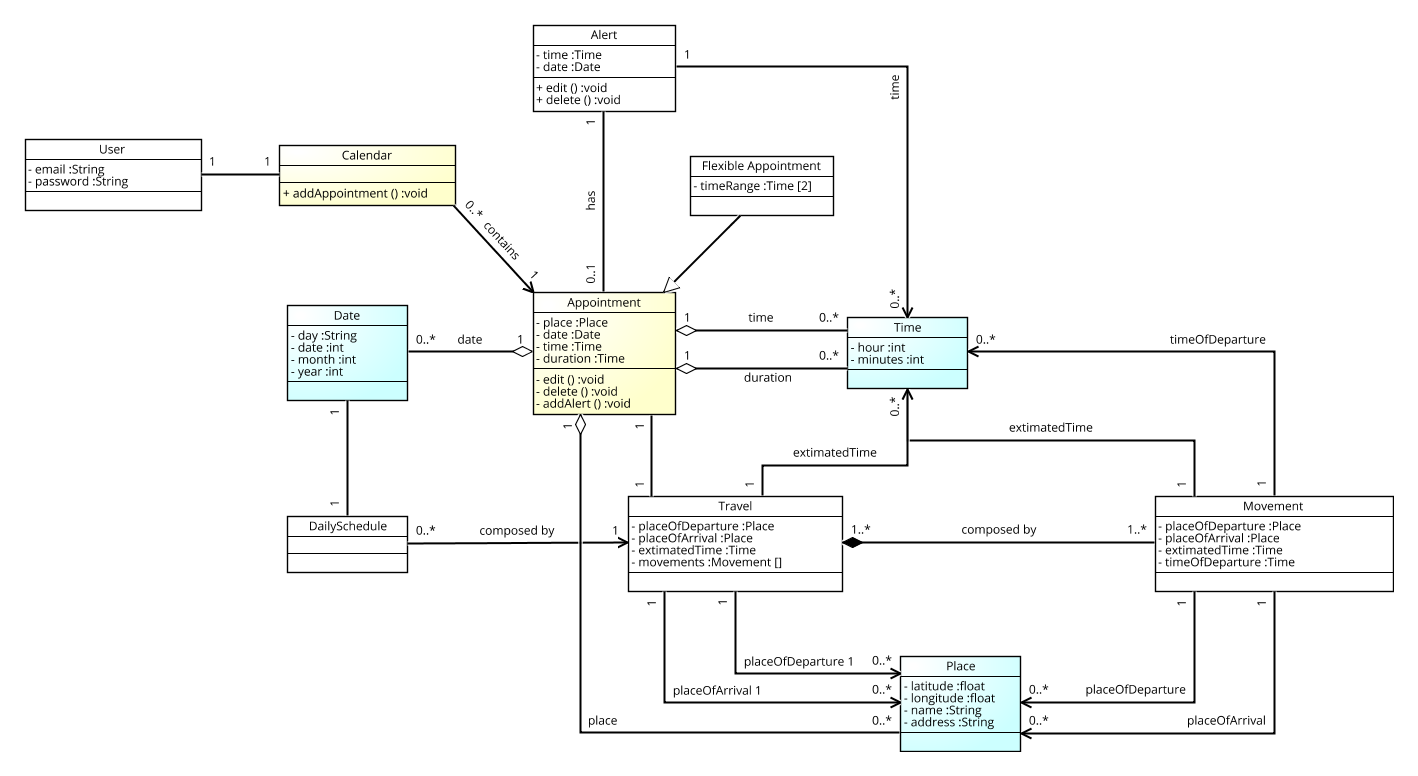
\includegraphics[width=1.2\textwidth]{Images/ClassDiagram.png}}%
\end{figure}

\subsection{Product functions}
This application aims to provide a smart and user-friendly appointment-manager system, which allows the user to create and keep track of several appointment on a personal virtual calendar. Plus, the app is able to schedule the travels to reach the different appointment destinations on time in the fastest and most confortable way, according to the preferences expressed by the user and the different weather and public transport condition. Finally, the application offers the possibility of easily buy tickets for the different trips, and to view them when needed.
\subsection{User characteristics}
We recommend this application to a everyone who wants to easily manage his appointments without any loss of time. The app is designed to be as user friendly as possible, so the user is not forced to have a specific knowledge of the system to be able to benefit of the service. It can be used by a business man with a calendar full of work meetings or just by an ordinary student to schedule his study breaks. Furthermore, the possibility of buying tickets suits even simple travelers who need to manage their trips.
\subsection{Dependencies}
\begin{itemize}
	\The application requires a stable internet connection, by Wi-Fi or mobile network.
	\The application makes use of GPS localization to access to the user position.
	\Based on the user choice, the application may require a connection to an existing Facebook or Google account.
	\The application makes use of external APIs to achieve information about maps, public transport and weather condition.
	\The application depends entirely on the ATM and Trenord public transport Payment Service for everything concerning the tickets purchase.
\end{itemize}
\subsection{Constrains}
\begin{itemize}
	\item The application requires the user to be registred and logged into the system to work properly.
	\item The application works only on smartphones that implement Android v. 4.0.3 or later.
	\item The application is in alpha version and works only inside the urban area of Milan.
	\item 30 Mb(?) of storage memory must be available on the device in order to correctly install the application.
\end{itemize}



	
	%------------------------------------------------------------------------------------------------------------------------------------------------
	\clearpage
	{\color{Blue}{\section{Specific Requirements}}}
	\label{sect:requirements}
	\subsection{External interface requirements}
\subsubsection{User interface}

\begin{figure}[!h]
	\centering
	\begin{minipage}[b]{0.65\textwidth}
		\makebox[\textwidth][c]{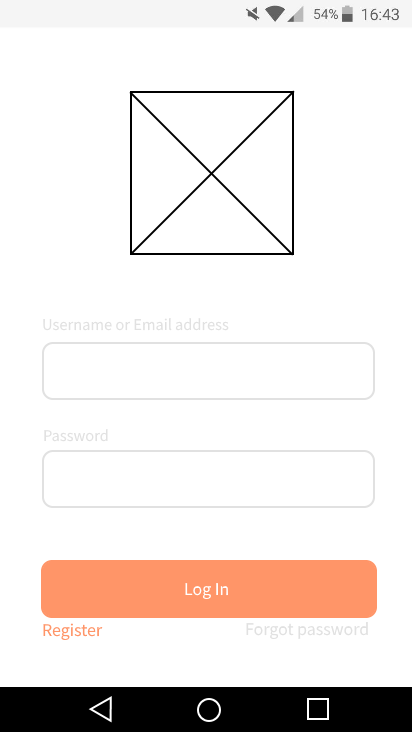
\includegraphics[width=0.50\textwidth]{Images/Mockup/LogPage.png}}%
		\caption{Login page}
	\end{minipage}
	\begin{minipage}[b]{0.65\textwidth}
		\makebox[\textwidth][c]{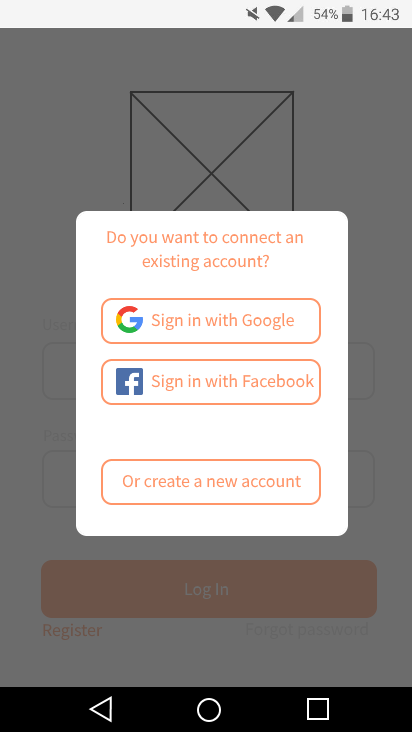
\includegraphics[width=0.50\textwidth]{Images/Mockup/GoogleConnectionPopup.png}}%
		\caption{Connection of an existent account}
	\end{minipage}
\end{figure}
\clearpage
\begin{figure}[!h]
	\centering
	\begin{minipage}[b]{0.65\textwidth}
		\makebox[\textwidth][c]{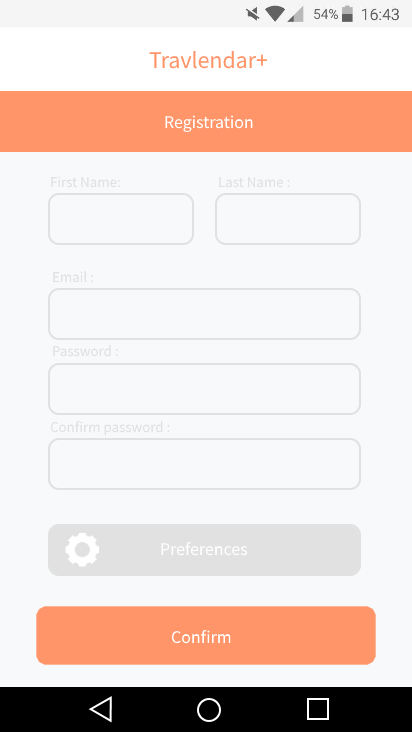
\includegraphics[width=0.50\textwidth]{Images/Mockup/RegistrationForm.png}}%
		\caption{Registration form}
	\end{minipage}
	\begin{minipage}[b]{0.65\textwidth}
		\makebox[\textwidth][c]{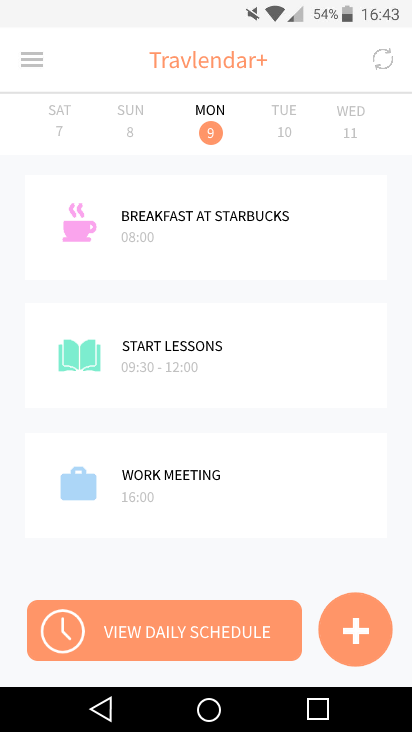
\includegraphics[width=0.50\textwidth]{Images/Mockup/Base.png}}%
		\caption{Daily view of calendar}
	\end{minipage}
\end{figure}
\clearpage
\begin{figure}[!h]
	\centering
	\begin{minipage}[b]{0.65\textwidth}
		\makebox[\textwidth][c]{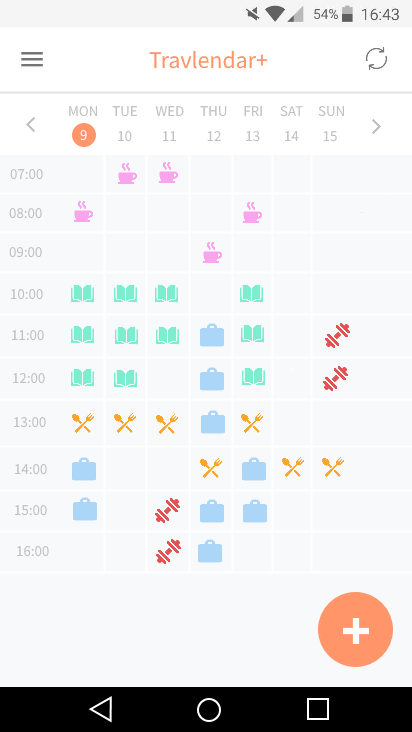
\includegraphics[width=0.50\textwidth]{Images/Mockup/Base3.png}}%
		\caption{Weekly view of calendar}
	\end{minipage}
	\begin{minipage}[b]{0.65\textwidth}
		\makebox[\textwidth][c]{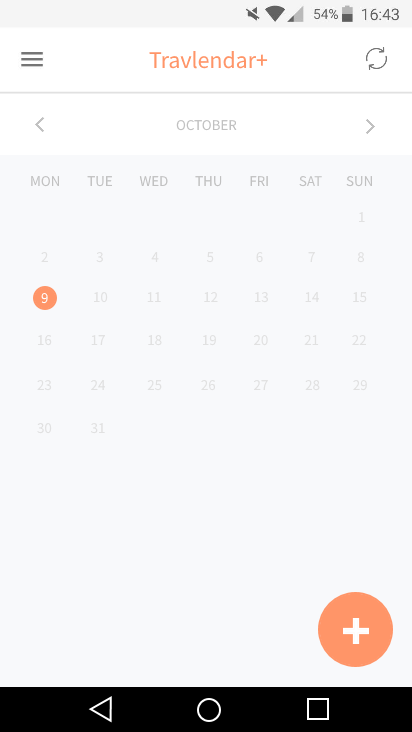
\includegraphics[width=0.50\textwidth]{Images/Mockup/Base2.png}}%
		\caption{Monthly view of calendar}
	\end{minipage}
\end{figure}
\clearpage
\begin{figure}[!h]
	\centering
	\begin{minipage}[b]{0.65\textwidth}
		\makebox[\textwidth][c]{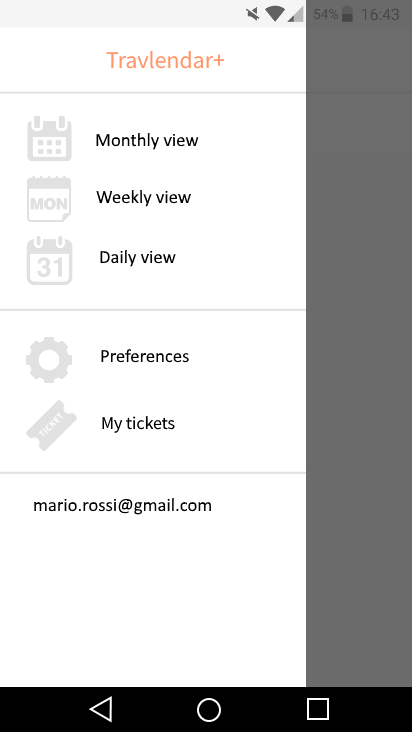
\includegraphics[width=0.50\textwidth]{Images/Mockup/LeftPanel.png}}%
		\caption{Menu}
	\end{minipage}
	\begin{minipage}[b]{0.65\textwidth}
		\makebox[\textwidth][c]{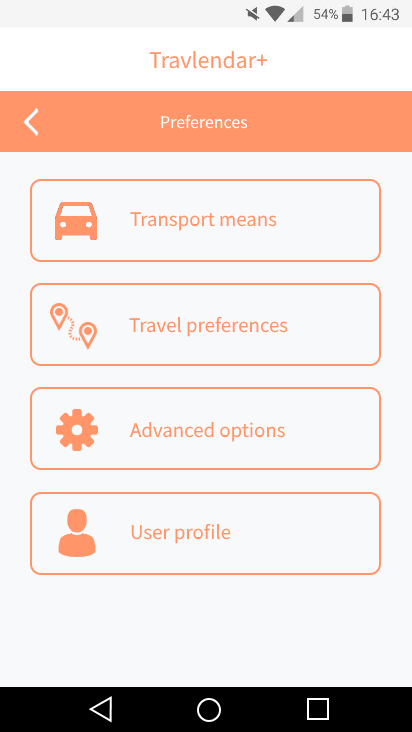
\includegraphics[width=0.50\textwidth]{Images/Mockup/PreferencesManager.png}}%
		\caption{Preferences menu}
	\end{minipage}
\end{figure}
\clearpage
\begin{figure}[!h]
	\centering
	\begin{minipage}[b]{0.65\textwidth}
		\makebox[\textwidth][c]{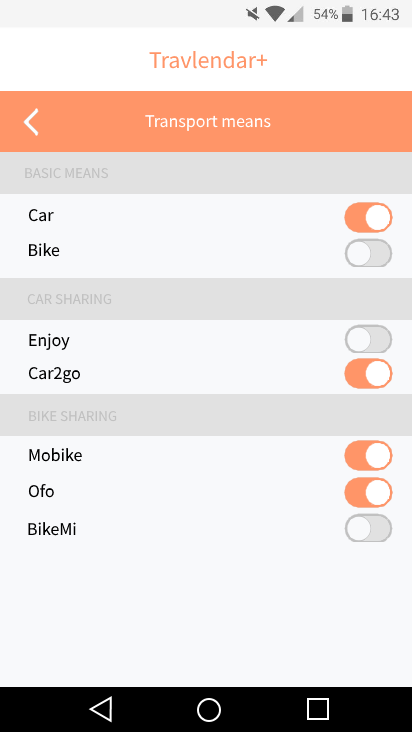
\includegraphics[width=0.50\textwidth]{Images/Mockup/transportMeansOpt.png}}%
		\caption{Transport means settings}
	\end{minipage}
	\begin{minipage}[b]{0.65\textwidth}
		\makebox[\textwidth][c]{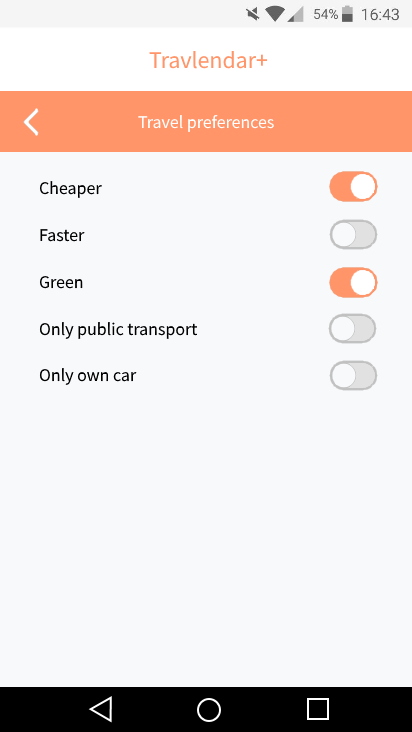
\includegraphics[width=0.50\textwidth]{Images/Mockup/TravelPreferences.png}}%
		\caption{Travel preferences}
	\end{minipage}
\end{figure}
\clearpage
\begin{figure}[!h]
	\centering
	\begin{minipage}[b]{0.65\textwidth}
		\makebox[\textwidth][c]{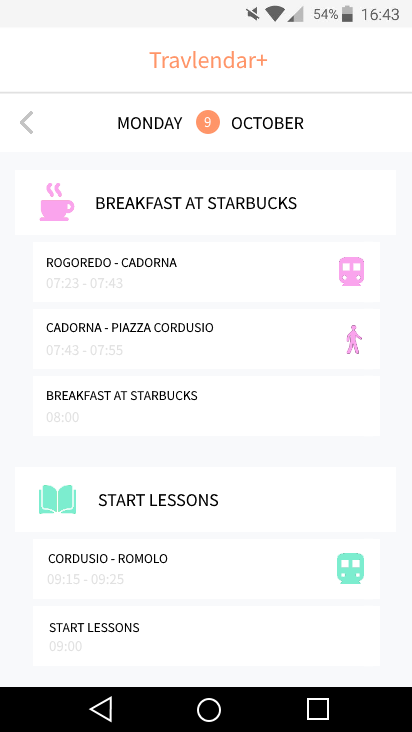
\includegraphics[width=0.50\textwidth]{Images/Mockup/DailySchedule.png}}%
		\caption{Daily schedule}
	\end{minipage}
	\begin{minipage}[b]{0.65\textwidth}
		\makebox[\textwidth][c]{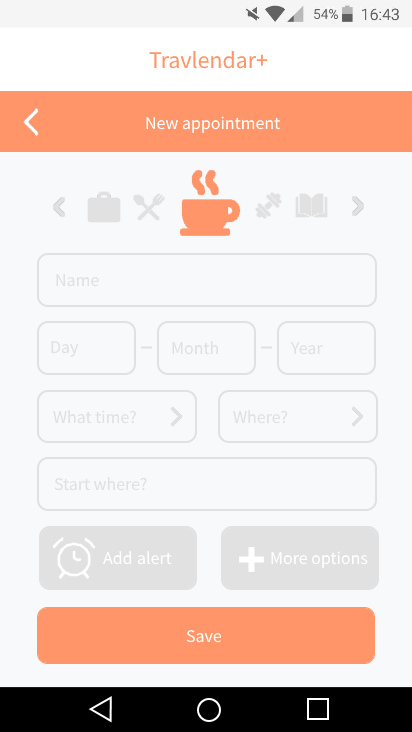
\includegraphics[width=0.50\textwidth]{Images/Mockup/EventCreator.png}}%
		\caption{New appointment}
	\end{minipage}
\end{figure}
\clearpage
\begin{figure}[!h]
	\centering
	\begin{minipage}[b]{0.65\textwidth}
		\makebox[\textwidth][c]{
\includegraphics[width=0.50\textwidth]{Images/Mockup/AlarmCreator.png}}%
		\caption{New alert}
	\end{minipage}
	\begin{minipage}[b]{0.65\textwidth}
		\makebox[\textwidth][c]{
\includegraphics[width=0.50\textwidth]{Images/Mockup/OptionPanel.png}}%
		\caption{appointment options}
	\end{minipage}
\end{figure}
\clearpage
\begin{figure}[!h]
	\centering
	\begin{minipage}[b]{0.65\textwidth}
		\makebox[\textwidth][c]{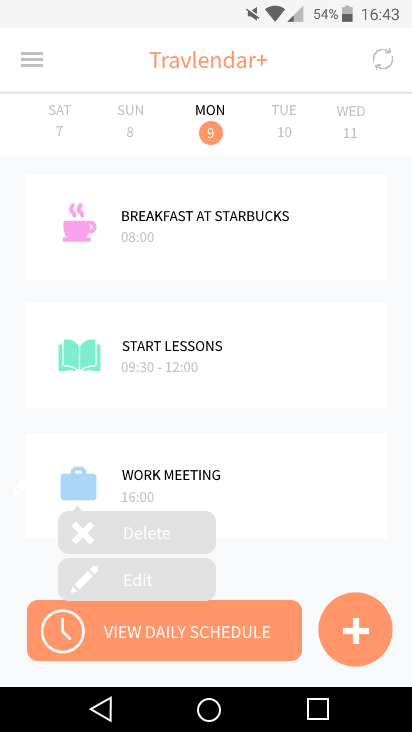
\includegraphics[width=0.50\textwidth]{Images/Mockup/BaseModificaDelete.png}}%
		\caption{Edit or delete appointment}
	\end{minipage}
	\begin{minipage}[b]{0.65\textwidth}
		\makebox[\textwidth][c]{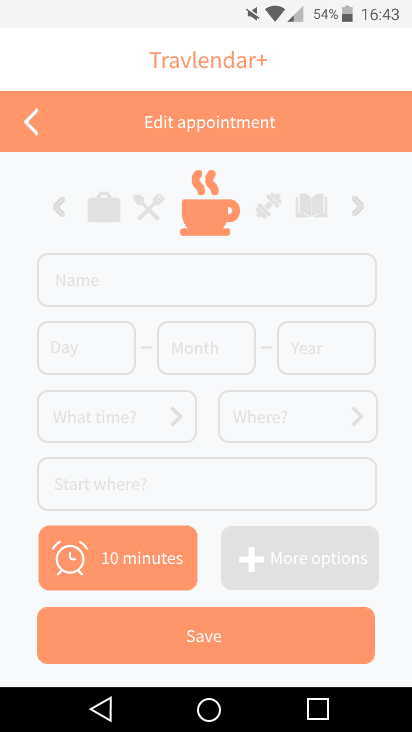
\includegraphics[width=0.50\textwidth]{Images/Mockup/EditAppointment.png}}%
		\caption{Edit appointment}
	\end{minipage}
\end{figure}
\clearpage
\begin{figure}[!h]
	\centering
	\begin{minipage}[b]{0.65\textwidth}
		\makebox[\textwidth][c]{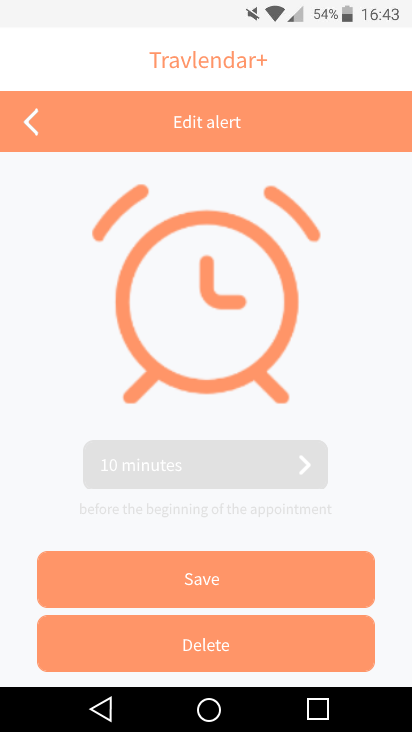
\includegraphics[width=0.50\textwidth]{Images/Mockup/AlarmEditDelete.png}}%
		\caption{Edit or delete alert}
	\end{minipage}
	\begin{minipage}[b]{0.65\textwidth}
		\makebox[\textwidth][c]{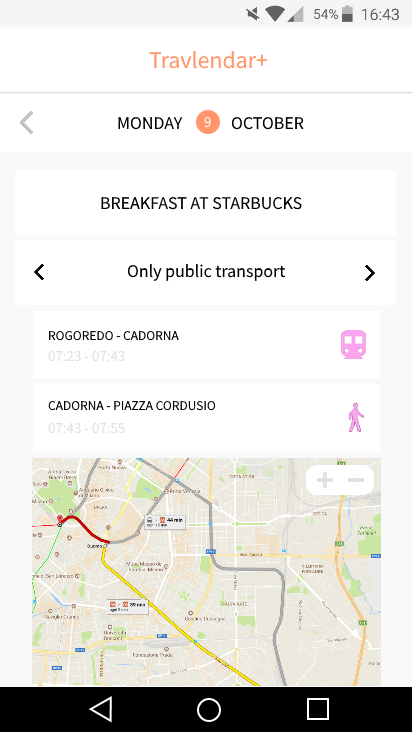
\includegraphics[width=0.50\textwidth]{Images/Mockup/TravelDetailsTrain.png}}%
		\caption{Travel details}
	\end{minipage}
\end{figure}
\clearpage
\begin{figure}[!h]
	\centering
	\begin{minipage}[b]{0.65\textwidth}
		\makebox[\textwidth][c]{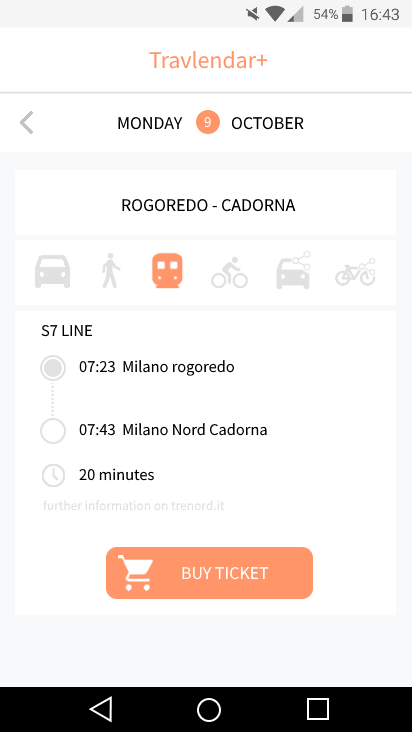
\includegraphics[width=0.50\textwidth]{Images/Mockup/MovementDetails.png}}%
		\caption{Movement details}
	\end{minipage}
\end{figure}

\subsubsection{Software interface}
The application makes uses of the following APIs:
\begin{itemize}
	\item Weather API: \href{url}{https://openweathermap.org/api}
	\item Google Maps API: \href{url}{https://developers.google.com/maps/}
	\item Trenord API: \href{url}{https://github.com/bluviolin/TrainMonitor/wiki/API-del-sistema-Viaggiatreno}
	\item Car2go API: \href{url}{https://github.com/car2go/openAPI}
	\item Enjoy API: \href{url}{https://github.com/mattiaongit/enjoy/blob/master/enjoy.py}
	\item BikeMi API: \href{url}{https://github.com/pierlauro/bikemi-unofficial-api}
	\item MoBike API: \href{url}{https://github.com/ubahnverleih/WoBike}
\end{itemize}
\clearpage
\subsection{Domain assumptions}
\begin{itemize}
	
\item \textbf{[D1]} The user is always connected via Internet and the connection is stable.
\item \textbf{[D2]} Information about weather, transport means, maps and travel times are provided by external APIs.
\item \textbf{[D3]} Data provided by external APIs are correct.
\item \textbf{[D4]} The process of ticket payment is made through an external public transport service.
\item \textbf{[D5]} If the payment is fulfilled without errors, the tickets are correctly received.

\end{itemize}

\subsection{Functional requirements}
\begin{itemize}
	\item \textbf{R1]} The user must be logged into the system to access application features.
	\item \textbf{[R2]} The user must be able to choose the option of creating a new appointment.
	\item \textbf{[R3]} The user must be able to choose the option of editing a selected appointment.
	\item \textbf{[R4]} The user must be able to choose the option of deleting a selected appointment.
	\item \textbf{[R5]} The system must be able to provide the user with an overview of his calendar and the user must be able to view all appointments fixed in a certain period.
	\item \textbf{[R6]} The user must be able to select a chosen day from the overview of his calendar.
	\item \textbf{[R7]} The user must be able to select a specific appointment in his calendar.
	\item \textbf{[R8]} The system must ask the user to provide all information needed for the creation of a new appointment, such as place and time of start and overall duration.
	\item \textbf{[R9]} The system must check if the information provided by the user are correct.
	\item \textbf{[R10]} The system must check if an appointment overlaps with other events and must eventually notify it to the user.
	\item \textbf{[R11]} The system must give the user access to all details of a selected appointment and the user must be allowed to edit the information needed.
	\item \textbf{[R12]} The user must be able to set advanced information for a created appointment.
	\item \textbf{[R13]} The user must be able to set an appointment as flexible, specifying the interval of time.
	\item \textbf{[R14]} The user must be able to set an appointment as repeatable, specifying the desired days.
	\item \textbf{[R15]} The system must schedule any flexible or repeatable appointment in the correct way, avoiding overlapping with other appointments.
	\item \textbf{[R16]} The appointment intended to be modified must have been previously successfully created and not already deleted.
	\item \textbf{[R17]} The user must confirm the creation of the new appointment.
	\item \textbf{[R18]} The user must confirm any appointment modification.
	\item \textbf{[R19]} The system must save the user modifications in memory and the calendar must be updated.
	\item \textbf{[R20]} The system must remove a deleted appointment from the memory and delete every alert related to it.
	\item \textbf{[R21]} The user must be able to switch between different possible calendar, such as daily calendar, weekly calendar and monthly calendar.
	\item \textbf{[R22]} The system must be able to provide information about the scheduled travels for a chosen day, showing the transport means and the estimated time required from each travel.
	\item \textbf{[R23]} The system must choose the best option between the possible travel alternatives according to the preferences expressed in the user profile settings and the information about external weather.
	\item \textbf{[R24]} The user must be able to select a specific travel in his daily schedule.
	\item \textbf{[R25]} The system must provide detailed information about the travels selected by the user, such as the trace route on the map and the weather conditions.
	\item \textbf{[R26]} The system must provide the user with an overview of the possible travel alternatives for the chosen travel, specifying all details for each one.
	\item \textbf{[R27]} The user must be able to filter the travel alternatives furnished by the system according to defined parameters, such as time of travelling or overall cost.
	\item \textbf{[R28]} The user must be able to choose a favourite travel option different from the displayed default one.
	\item \textbf{[R29]} The user must be able to select a specific movement in a travel.
	\item \textbf{[R30]} The system must provide detailed information about the movements selected by the user, such as the specific trace route on the map and the price of the ticket.
	\item \textbf{[R31]} The user must be able to choose an alternative transport mean for a selected movement, if there are any.
	\item \textbf{[R32]} The system must update the daily schedule according to the travel option chosen by the user and the user must be able to see the new updated schedule.
	\item \textbf{[R33]} The system must give to the user the possibility of buying the ticket for the selected travel.
	\item \textbf{[R34]} The system must save a copy of the bought tickets.
	\item \textbf{[R35]} The user must be able to access to a ticket page from the home page.
	\item \textbf{[R36]} The system must provide a list of all the bought tickets and the user must be able to select and view a specific one in full screen.
	\item \textbf{[R37]} The user must be able to access the preferences panel of his account.
	\item \textbf{[R38]} The system must give the user the possibility of setting various preferences, such as owned and preferred travel means, address of Home and other general travel preferences.
	\item \textbf{[R39]} The user must be able to edit the provided preferences when needed.
	\item \textbf{[R40]} The system must give the user the possibility of adding an alert to an appointment while it is being created or modified.
	\item \textbf{[R41]} The user must be able to choose a desired interval of time for the warning alert.
	\item \textbf{[R42]} The user must confirm the alert creation and the system must save the insertion in the memory.
	\item \textbf{[R43]} The user must be able to modify or remove the inserted alert when needed.
	\item \textbf{R44]} In case of any alert modification made by the user, the user must confirm the modification and the system must save all changes.
	
\end{itemize}

\subsection{Goals}
\subsubsection{[G1] Allow an User to create a new appointment in his calendar.}
\begin{itemize}
	\item \textbf{[R1]} The user must be logged into the system to access application features.
	\item \textbf{[R5]} The system must be able to provide the user with an overview of his calendar and the user must be able to view all appointments fixed in a certain period.
	\item \textbf{[R6]} The user must be able to select a chosen day from the overview of his calendar.
	\item \textbf{[R2]} The user must be able to choose the option of creating a new appointment.
	\item \textbf{[R8]} The system must ask the user to provide all information needed for the creation of a new appointment, such as place and time of start and overall duration.
	\item \textbf{[R40]} The system must give the user the possibility of adding an alert to an appointment while it is being created or modified.
	\item \textbf{[R9]} The system must check if the information provided by the user are correct.
	\item \textbf{[R12]} The user must be able to set advanced information for a created appointment.
	\item \textbf{[R10]} The system must check if an appointment overlaps with other events and must eventually notify it to the user.
	\item \textbf{[R17]} The user must confirm the creation of the new appointment.
	\item \textbf{[R19]} The system must save the user modifications in memory and the calendar must be updated.
\end{itemize}

\subsubsection{[G2] Allow a user to create flexible and repeatable appointments (such as lunches, study breaks etc.)}
\begin{itemize}
	\item \textbf{[R1]} The user must be logged into the system to access application features.
	\item \textbf{[R2]} The user must be able to choose the option of creating a new appointment.
	\item \textbf{[R12]} The user must be able to set advanced information for a created appointment.
	\item \textbf{[R13]} The user must be able to set an appointment as flexible, specifying the interval of time.
	\item \textbf{[R14]} The user must be able to set an appointment as repeatable, specifying the desired days.
	\item \textbf{[R15]} The system must schedule any flexible or repeatable appointment in the correct way, avoiding overlapping with other appointments.	
\end{itemize}

\subsubsection{[G3] Allow a user to edit an existing appointment in his calendar.}
\begin{itemize}
	\item \textbf{[R1]} The user must be logged into the system to access application features.
	\item \textbf{[R16]} The appointment intended to be modified must have been previously successfully created and not already deleted.
	\item \textbf{[R5]} The system must be able to provide the user with an overview of his calendar and the user must be able to view all appointments fixed in a certain period.
	\item \textbf{[R7]} The user must be able to select a specific appointment in his calendar.
	\item \textbf{[R3]} The user must be able to choose the option of editing a selected appointment.
	\item \textbf{[R11]} The system must give the user access to all details of a selected appointment and the user must be allowed to edit the information needed.
	\item \textbf{[R40]} The system must give the user the possibility of adding an alert to an appointment while it is being created or modified.
	\item \textbf{[R9]} The system must check if the information provided by the user are correct.
	\item \textbf{[R10]} The system must check if an appointment overlaps with other events and must eventually notify it to the user.
	\item \textbf{[R18]} The user must confirm any appointment modification.
	\item \textbf{[R19]} The system must save the user modifications in memory and the calendar must be updated.
\end{itemize}

\subsubsection{[G4] Allow a user to delete an existing appointment from his calendar.}
\begin{itemize}
	\item \textbf{[R1]} The user must be logged into the system to access application features.
	\item \textbf{[R5]} The system must be able to provide the user with an overview of his calendar and the user must be able to view all appointments fixed in a certain period.
	\item \textbf{[R16]} The appointment intended to be modified must have been previously successfully created and not already deleted.
	\item \textbf{[R7]} The user must be able to select a specific appointment in his calendar.
	\item \textbf{[R4]} The user must be able to choose the option of deleting a selected appointment.
	\item \textbf{[R18]} The user must confirm any appointment modification.
	\item \textbf{[R20]} The system must remove a deleted appointment from the memory and delete every alert related to it.
	\item \textbf{[R19]} The system must save the user modifications in memory and the calendar must be updated.	
\end{itemize}

\subsubsection{[G5] Allow a user to check his calendar to see his appointments.}
\begin{itemize}
	\item \textbf{[R1]} The user must be logged into the system to access application features. 
	\item \textbf{[R5]} The system must be able to provide the user with an overview of his calendar and the user must be able to view all appointments fixed in a certain period.
	\item \textbf{[R21]} The user must be able to switch between different possible calendar, such as daily calendar, weekly calendar and monthly calendar.
\end{itemize}

\subsubsection{[G6] Allow a user to view his Daily Schedule.}
\begin{itemize}
	\item \textbf{[R1]} The user must be logged into the system to access application features.
	\item \textbf{[R6]} The user must be able to select a chosen day from the overview of his calendar.
	\item \textbf{[R22]} The system must be able to provide information about the scheduled travels for a chosen day, showing the transport means and the estimated time required from each travel.
	\item \textbf{[R23]} The system must choose the best option between the possible travel alternatives according to the preferences expressed in the user profile settings and the information about external weather.
	\item \textbf{[D1]} The user is always connected via Internet and the connection is stable.
	\item \textbf{[D2]} Information about weather, transport means, maps and travel times are provided by external APIs.
	\item \textbf{[D3]} Data provided by external APIs are correct.
\end{itemize}

\subsubsection{[G7] Allow a user to see all the details of a specific travel.}
\begin{itemize}
	\item \textbf{[R1]} The user must be logged into the system to access application features.
	\item \textbf{[R22]} The system must be able to provide information about the scheduled travels for a chosen day, showing the transport means and the estimated time required from each travel.
	\item \textbf{[R24]} The user must be able to select a specific travel in his daily schedule.
	\item \textbf{[R25]} The system must provide detailed information about the travels selected by the user, such as the trace route on the map and the weather conditions.
	\item \textbf{[R29]} The user must be able to select a specific movement in a travel.
	\item \textbf{[R30]} The system must provide detailed information about the movements selected by the user, such as the specific trace route on the map and the price of the ticket.
	\item \textbf{[D1]} The user is always connected via Internet and the connection is stable.
	\item \textbf{[D2]} Information about weather, transport means, maps and travel times are provided by external APIs.
	\item \textbf{[D3]} Data provided by external APIs are correct.
\end{itemize}

\subsubsection{[G8] Allow a user to navigate and choose between different travel alternatives.}
\begin{itemize}
	\item \textbf{[R1]} The user must be logged into the system to access application features. 
	\item \textbf{[R24]} The user must be able to select a specific travel in his daily schedule.
	\item \textbf{[R26]} The system must provide the user with an overview of the possible travel alternatives for the chosen travel, specifying all details for each one.
	\item \textbf{[R27]} The user must be able to filter the travel alternatives furnished by the system according to defined parameters, such as time of travelling or overall cost.
	\item \textbf{[R28]} The user must be able to choose a favourite travel option different from the displayed default one.
	\item \textbf{[R29]} The user must be able to select a specific movement in a travel.
	\item \textbf{[R31]} The user must be able to choose an alternative transport mean for a selected movement, if there are any.
	\item \textbf{[R32]} The system must update the daily schedule according to the travel option chosen by the user and the user must be able to see the new updated schedule.
	\item \textbf{[D1]} The user is always connected via Internet and the connection is stable.
	\item \textbf{[D2]} Information about weather, transport means, maps and travel times are provided by external APIs.
	\item \textbf{[D3]} Data provided by external APIs are correct.
\end{itemize}

\subsubsection{[G9] Allow a user to manage alerts for each appointment.}
\begin{itemize}
	\item \textbf{[R40]} The system must give the user the possibility of adding an alert to an appointment while it is being created or modified.
	\item \textbf{[R41]} The user must be able to choose a desired interval of time for the warning alert.
	\item \textbf{[R42]} The user must confirm the alert creation and the system must save the insertion in the memory.
	\item \textbf{[R43]} The user must be able to modify or remove the inserted alert when needed.
	\item \textbf{[R44]} In case of any alert modification made by the user, the user must confirm the modification and the system must save all changes.
\end{itemize}

\subsubsection{[G10] Allow a user to manage his travel preferences.}
\begin{itemize}
	\item \textbf{[R37]} The user must be able to access the preferences panel of his account from the home page.
	\item \textbf{[R38]} The system must give the user the possibility of setting various preferences, such as owned and preferred travel means, address of Home and other general travel preferences.
	\item \textbf{[R39]} The user must be able to edit the provided preferences when needed.	
\end{itemize}

\subsubsection{[G11] Allow a user to buy public transportation tickets.}
\begin{itemize}
	\item \textbf{[R1]} The user must be logged into the system to access application features.
	\item \textbf{[R29]} The user must be able to select a specific movement in a travel.
	\item \textbf{[R33]} The system must give to the user the possibility of buying the ticket for the selected travel.
	\item \textbf{[R34]} The system must save a copy of the bought tickets.
	\item \textbf{[D5]} The payment process and ticket acquisition is made by an external public transport service.
	\item \textbf{[D1]} The user is always connected via Internet and the connection is stable.
	\item \textbf{[D4]} The process of ticket payment is made through an external public transport service.
	\item \textbf{[D5]} If the payment is fulfilled without errors, the tickets are correctly received.
\end{itemize}

\subsubsection{[G12] Allow a user to view the previously bought tickets.}
\begin{itemize}
	\item \textbf{[R1]} The user must be logged into the system to access application features.
	\item \textbf{[R34]} The system must save a copy of the bought tickets.
	\item \textbf{[R35]} The user must be able to access to a ticket page from the home page.
	\item \textbf{[R36]} The system must provide a list of all the bought tickets and the user must be able to select and view a specific one in full screen.	
\end{itemize}

\subsection{Design constraints}
\subsubsection{Standards compliance}
The application must require to the user different permissions:
\begin{itemize}
	\item Access to the calendar;
	\item Get hit position with GPS;
	\item Access to device storage.
\end{itemize}
\subsubsection{Hardware limitations}
The application, at the moment, runs only on Android 4.0.3 version or newer. \\
The device needs:
\begin{itemize}
	\item Internet connection;
	\item GPS;
	\item Space for save application in memory.
\end{itemize}
Actual devices on the market satisfy all these requirements.
\subsection{Software system attributes}
\subsubsection{Reliability}
The system must guarantee a 24/7 service.
\subsubsection{Availability}
The system requires a GPS service and internet connection in order to work properly. When the connection is down the system works with the last updated information available in the device memory.  
\subsubsection{Security}
The application must provide secure storage for all sensitive data inserted by the user. One way to achieve it is the use of cryptographical techniques.
\subsubsection{Maintainability}
The application will be released in beta version, meaning that it may eventually have some bugs. The application will be periodically upgraded and each release will be focus on solving detected problems.
Periodically all information stored in the application must be backed up, in order to reduce the possibility of losing information in case of malfunctions.
\subsubsection{Portability}
The application will be released only for Android smartphones (more specifically only for Android version 4.0.3 Ice Cream Sandwich or later).\\
Future plan is to lead the software also on iOS devices.


	
	%------------------------------------------------------------------------------------------------------------------------------------------------
	\clearpage
	{\color{Blue}{\section{Scenarios}}}
	\label{sect:scenarios}
	\subsection{Scenario 1}
Andrea has just booked a last minute flight from Milan Orio al Serio airport to Prague, in Czech Republic, but being not a frequent flyer, he’s pretty worried about the idea of losing his plane. Furthermore, he lives far away from the airport and he needs to reach it by public transportation. Two days before his departure, he decides to download Travlendar+ app. He creates a new account by connetting his Facebook profile and fills out the essential account settings, giving his basic preferences (he doesn’t have any car or bike and he prefers cheaper travels). Then he creates a new appointment called “Prague”in his calendar, inserting the date of Saturday 11/11/17, the time 13:00 and the location of the airport. He chooses the option “I want to be there…” and select “2 hours before”. Then he creates the new appointment. His calendar now shows the “Prague” event, and the app easily displays how to reach the airport in time, by leaving home at 9:32, walking until the nearest metro station, taking the metro until Stazione Centrale and then taking a public bus to the airport at 10:10. Now Andrea feels much more confident!
\subsection{Scenario 2}
Serena has been using the Travlendar+ app since a couple of weeks. She has just bought a new car that allows her to move trough the city in a easier way, and wants the app to consider that when it display the optimal travel solution. She opens the app and moves to the preferences panel of her account. She then select “Travel means owned” and puts a tick in the “car” option. Then, she open her calendar and check her daily schedules for the next three days. Some of the travels suggested by the app are now changed and replaced with faster and more confortable movements with car.
\subsection{Scenario 3}
Marco has a scheduled appointment in program for the following day, and the app used to suggest a 7 minutes-movement by bike until the train station. But now the weather widget seems to announce a rainy day, and the app switched to a warmer travel by metro. But Marco is not afraid of rain and likes walking, so he opens the daily schedule, selects the metro movement and checks the possible travel alternatives. He then chooses the option “by walk”. The app nows shows the updated schedule, and the system will remember the choice for the future.
\subsection{Scenario 4}
Riccardo is a pretty absent-minded man, and has a morning full of appointments in schedule for the next day. He has added all the meetings in his calendar, but must absolutely not forget them, so he decides to add an alarm to each of them, in order to remember his commitments. He opens the app and select one by one all his appointments of Tuesday. For each one, he taps on “add an alert to this appointment” and chooses to be warned 15 minutes before the start. 
	
	%------------------------------------------------------------------------------------------------------------------------------------------------
	\clearpage
	{\color{Blue}{\section{UML modelling}}}
	\label{sect:UMLmodelling}
	\subsection{Use case}
\begin{figure}[!h]
	\centering
	\makebox[\textwidth][c]{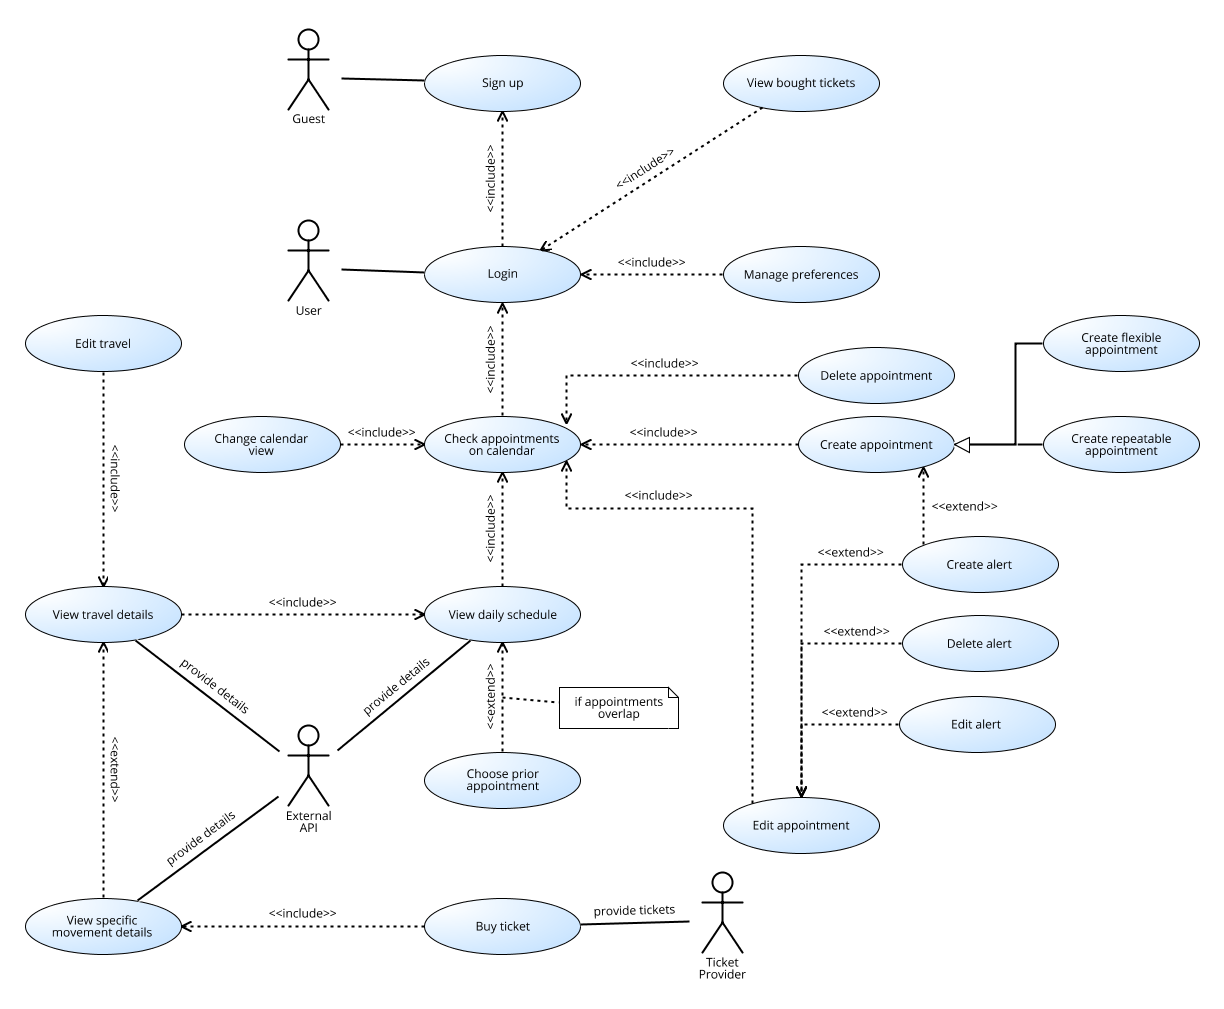
\includegraphics[width=1.2\textwidth]{Images/UseCaseDiagram.png}}%
	\caption{Use case diagram}
\end{figure}
\clearpage

\subsubsection{Sign up}
\begin{table}[!h]
	\centering
	{\renewcommand{\arraystretch}{2}%
		\begin{tabular}{|l|p{12cm}|}
			\hline
			\textbf{Name} 				& \textbf{Sign up} \\ \hline
			\textbf{Actors} 			& Guest \\ \hline
			\textbf{Entry conditions} 	& The guest is on the log in page of the application and clicks on “Register” button. \\ \hline
			\textbf{Flow of events}		& \begin{minipage}[t]{0.75\textwidth}
				\begin{enumerate}
					\item A pop-up shows up asking to the guest if he wants to connect an existing account, such as Google or Facebook, or if he want to create a new account.
					\begin{enumerate}
						\item If the guest connects his account, the system accepts the request and creates a new Travlendar+ account based on provided account.
						\item If the guest chooses to create a new account, he is redirected to the registration page which contains all the fields to be filled.
					\end{enumerate}
					\item The guest fills out all the mandatory fields.
					\item (Optional) The guest adjusts the preferences settings.
					\item The guest clicks on button “Confirm”.
					\item The system checks data provided and eventually creates and registers the user account.
				\end{enumerate}
			\end{minipage}	\\ \hline
			\textbf{Exit conditions}	& The guest has successfully created a new account and he can log into the system with his credentials. \\ \hline
			\textbf{Exceptions}			& \begin{minipage}[t]{0.75\textwidth}
				\begin{itemize}
					\item Email provided is already in use. The system does not proceed in the registration process and the account is not created. It is possible to repeat the procedure.
					\item Data provided are incorrect. The system highlights the incorrect fields and asks the user to repeat the procedure.
				\end{itemize} 
			\end{minipage} \\ \hline
	\end{tabular}}
\end{table}
\clearpage

\subsubsection{Log in}
\begin{table}[!h]
	\centering
	{\renewcommand{\arraystretch}{2}%
		\begin{tabular}{|l|p{12cm}|}
			\hline
			\textbf{Name} 				& \textbf{Log in} \\ \hline
			\textbf{Actors} 			& User \\ \hline
			\textbf{Entry conditions} 	& The user launches the application and clicks on the “Log In” button. \\ \hline
			\textbf{Flow of events}		& \begin{minipage}[t]{0.75\textwidth}
				\begin{enumerate}
					\item The user inserts his email.
					\item The user inserts his password.
					\item The user clicks on the “Log In” button.
				\end{enumerate}
			\end{minipage}	\\ \hline
			\textbf{Exit conditions}	& The login procedure is successfully completed. The user is logged into the system and is able to access to all the functionalities. \\ \hline
			\textbf{Exceptions}			& The credentials provided are not associated to any existing account. The login procedure is rejected and the guest is brought back to the login page. It is possible to repeat the procedure. \\ \hline
	\end{tabular}}
\end{table}

\subsubsection{Manage preferences}
\begin{table}[!h]
	\centering
	{\renewcommand{\arraystretch}{2}%
		\begin{tabular}{|l|p{12cm}|}
			\hline
			\textbf{Name} 				& \textbf{Manage preferences} \\ \hline
			\textbf{Actors} 			& User \\ \hline
			\textbf{Entry conditions} 	& The user clicks on “Preferences” from the side menu on the homepage. \\ \hline
			\textbf{Flow of events}		& \begin{minipage}[t]{0.75\textwidth}
				\begin{enumerate}
					\item The system shows the preferences settings, that include transport means owned, favorite kind of travel and other advanced options.
					\item The user accesses to the desired settings and adjusts the preferences as wanted.
					\item The user saves the changes.
				\end{enumerate}
			\end{minipage}	\\ \hline
			\textbf{Exit conditions}	& The changes are saved and remembered from the system. The preferences have been updated.  \\ \hline
			\textbf{Exceptions}			& The user clicks on “back” without having confirmed the creation. The new preferences are not saved and the application returns to the homepage. It is possible to repeat the procedure. \\ \hline
	\end{tabular}}
\end{table}
\clearpage

\subsubsection{View daily schedule}
\begin{table}[!h]
	\centering
	{\renewcommand{\arraystretch}{2}%
		\begin{tabular}{|l|p{12cm}|}
			\hline
			\textbf{Name} 				& \textbf{View daily schedule} \\ \hline
			\textbf{Actors} 			& User, External APIs \\ \hline
			\textbf{Entry conditions} 	& The user clicks on the “View daily schedule” button while checking an appointment on his calendar. \\ \hline
			\textbf{Flow of events}		& \begin{minipage}[t]{0.75\textwidth}
				\begin{enumerate}
					\item The system receives data from different external APIs about routes, traffic, weather and available transport means and computes the best travel option according to the user preferences.
					\item The system provides a graphic overview of all the travels scheduled for the day, with the relative movements.
					\item The user checks all the information needed and eventually clicks on a specific travel or movement to get further information.
				\end{enumerate}
			\end{minipage}	\\ \hline
			\textbf{Exit conditions}	& User has obtained all the information needed and has clicked “back” to return to the homepage or has selected a specific travel/movement to get further information.  \\ \hline
			\textbf{Exceptions}			& \begin{minipage}[t]{0.75\textwidth}
				\begin{itemize}
					\item Some of the appointments overlap. The system is not able to compute travels between the appointments and forces the user to choose a prior appointment.
					\item Some of the appointments are not reachable in the allotted time. The system doesn’t show the travel and signals the problem to the user with a warning.
				\end{itemize} 
			\end{minipage} \\ \hline
	\end{tabular}}
\end{table}
\clearpage

\subsubsection{View travel details}
\begin{table}[!h]
	\centering
	{\renewcommand{\arraystretch}{2}%
		\begin{tabular}{|l|p{12cm}|}
			\hline
			\textbf{Name} 				& \textbf{View travel details} \\ \hline
			\textbf{Actors} 			& User, External APIs \\ \hline
			\textbf{Entry conditions} 	& The user is checking his daily schedule and clicks on a specific travel. \\ \hline
			\textbf{Flow of events}		& \begin{minipage}[t]{0.75\textwidth}
				\begin{enumerate}
					\item The system receives data from different external APIs and collects detailed information about the travel, such as the specific itinerary on the map and the weather conditions.
					\item The user is redirected to a new page that displays all the information about the selected travel.
					\item The user checks all the information needed and eventually clicks on a specific movement to get further information or buy a ticket.
				\end{enumerate}
			\end{minipage}	\\ \hline
			\textbf{Exit conditions}	& User has obtained all the information needed and has clicked “back” to return to the daily schedule or has selected a specific movement to get further information.  \\ \hline
			\textbf{Exceptions}			& No exceptions expected  \\ \hline
	\end{tabular}}
\end{table}

\subsubsection{Edit travel}
\begin{table}[!h]
	\centering
	{\renewcommand{\arraystretch}{2}%
		\begin{tabular}{|l|p{12cm}|}
			\hline
			\textbf{Name} 				& \textbf{Edit travel} \\ \hline
			\textbf{Actors} 			& User \\ \hline
			\textbf{Entry conditions} 	& The user is checking a specific travel. \\ \hline
			\textbf{Flow of events}		& \begin{minipage}[t]{0.75\textwidth}
				\begin{enumerate}
					\item The user provides modifications to the travel as followed:
					\begin{enumerate}
						\item Clicking on the travel preferences and switching to a different alternative.
						\item Clicking on a specific movement and changing the transport mean.
					\end{enumerate}
					\item The user saves the changes.
				\end{enumerate}
			\end{minipage}	\\ \hline
			\textbf{Exit conditions}	& The changes are saved and the system displays the new modified travel.   \\ \hline
			\textbf{Exceptions}			& There are no possible alternatives for the selected travel. The system displays a warning to notify the user.  \\ \hline
	\end{tabular}}
\end{table}

\subsubsection{View specific movement details}
\begin{table}[!h]
	\centering
	{\renewcommand{\arraystretch}{2}%
		\begin{tabular}{|l|p{12cm}|}
			\hline
			\textbf{Name} 				& \textbf{View specific movement details} \\ \hline
			\textbf{Actors} 			& User \\ \hline
			\textbf{Entry conditions} 	& User is checking a specific travel and select a specific movement. \\ \hline
			\textbf{Flow of events}		& \begin{minipage}[t]{0.75\textwidth}
				\begin{enumerate}
					\item The system receives data from different external APIs and collects detailed information about the movement, such as the specific itinerary on the map, the weather conditions and the eventual availability of tickets.
					\item The user is redirected to a new page that displays all the information about the selected movement.
					\item The user checks all the information needed and eventually proceeds in buying a ticket.
				\end{enumerate}
			\end{minipage}	\\ \hline
			\textbf{Exit conditions}	& User has obtained all the information needed and has clicked “back” to return to the travel page or has proceeded in buying a ticket.  \\ \hline
			\textbf{Exceptions}			& No exceptions expected  \\ \hline
	\end{tabular}}
\end{table}

\subsubsection{Choose prior appointment}
\begin{table}[!h]
	\centering
	{\renewcommand{\arraystretch}{2}%
		\begin{tabular}{|l|p{12cm}|}
			\hline
			\textbf{Name} 				& \textbf{Choose prior appointment} \\ \hline
			\textbf{Actors} 			& User \\ \hline
			\textbf{Entry conditions} 	& The user is checking the schedule and two appointments overlap. \\ \hline
			\textbf{Flow of events}		& \begin{minipage}[t]{0.75\textwidth}
				\begin{enumerate}
					\item The system signals the user the exactly time overlapping of the appointments.
					\item The user clicks on the preferred appointment.
					\item The system re-computes the daily schedule giving priority to the chosen appointment.
				\end{enumerate}
			\end{minipage}	\\ \hline
			\textbf{Exit conditions}	& No more appointments overlap. The system shows the daily schedule without errors.  \\ \hline
			\textbf{Exceptions}			& No exceptions expected  \\ \hline
	\end{tabular}}
\end{table}
\clearpage

\subsubsection{Buy ticket}
\begin{table}[!h]
	\centering
	{\renewcommand{\arraystretch}{2}%
		\begin{tabular}{|l|p{12cm}|}
			\hline
			\textbf{Name} 				& \textbf{Buy ticket} \\ \hline
			\textbf{Actors} 			& User, Ticket provider \\ \hline
			\textbf{Entry conditions} 	& User is checking a specific movement and clicks on “Buy ticket” \\ \hline
			\textbf{Flow of events}		& \begin{minipage}[t]{0.75\textwidth}
				\begin{enumerate}
					\item The system connects trough APIs to the external system of the ticket provider.
					\item The system shows the user a form to fill with all the payment information.
					\item The user fills out all the fields and confirm the payment.
					\item The system sends information to the ticket provider and waits for confirmation and ticket data.
				\end{enumerate}
			\end{minipage}	\\ \hline
			\textbf{Exit conditions}	& Payment is successfully fulfilled and bought tickets are available for the view. The user is brought back to the movement page.  \\ \hline
			\textbf{Exceptions}			& Payment is rejected. The system notifies the user with a warning. It is possible to repeat the procedure. \\ \hline
	\end{tabular}}
\end{table}
\clearpage

\subsubsection{Delete appointment}
\begin{table}[!h]
	\centering
	{\renewcommand{\arraystretch}{2}%
		\begin{tabular}{|l|p{12cm}|}
			\hline
			\textbf{Name} 				& \textbf{Delete appointment} \\ \hline
			\textbf{Actors} 			& User \\ \hline
			\textbf{Entry conditions} 	& The user selects a specific appointment in his calendar (through daily or weekly view) and clicks on “Delete” button. \\ \hline
			\textbf{Flow of events}		& \begin{minipage}[t]{0.75\textwidth}
				\begin{enumerate}
					\item A pop-up shows up, asking the user to confirm the deletion.
					\item The user confirms the deletion.
					\item The system removes all the appointment information from the memory, alert included.
				\end{enumerate}
			\end{minipage}	\\ \hline
			\textbf{Exit conditions}	& The appointment has been deleted and removed from the system. The user is redirected to his calendar page, which has been updated with the removal of the appointment.  \\ \hline
			\textbf{Exceptions}			& The user does not confirm the deletion. The appointment has not been deleted and the user is redirected to his calendar page. It is possible to repeat the procedure.  \\ \hline
	\end{tabular}}
\end{table}
\clearpage

\subsubsection{Create appointment}
\begin{table}[!h]
	\centering
	{\renewcommand{\arraystretch}{2}%
		\begin{tabular}{|l|p{12cm}|}
			\hline
			\textbf{Name} 				& \textbf{Create appointment} \\ \hline
			\textbf{Actors} 			& User \\ \hline
			\textbf{Entry conditions} 	& The user is checking his calendar and clicks on “Create appointment” button. \\ \hline
			\textbf{Flow of events}		& \begin{minipage}[t]{0.75\textwidth}
				\begin{enumerate}
					\item The user is redirected to the appointment creation page, which contains all the fields required to perform the creation.
					\item The user fills out all mandatory fields.
					The following steps aren’t mandatory:
					\begin{enumerate}
						\item User chooses among the available icons.
						\item User adds an alert to remember the appointment.
						\item User clicks on “More options” and provides more detailed options.
					\end{enumerate}
					\item User confirms the creation.
					\item The system saves the appointment information.
				\end{enumerate}
			\end{minipage}	\\ \hline
			\textbf{Exit conditions}	& The appointment is created and inserted in the system. The user is redirected to his calendar page, which has been updated with the new appointment.  \\ \hline
			\textbf{Exceptions}			& \begin{minipage}[t]{0.75\textwidth}
				\begin{itemize}
					\item The user has provided incorrect information: the appointment is not created and the user must repeat the procedure. 
					\item The user clicks on “back” without having confirmed the creation. The appointment is not created and the application returns to the calendar page. It is possible to repeat the procedure.
					\item The appointment overlaps with other previously created appointments. The appointment is created and inserted anyway, but the user receives a notification of the overlapping.
				\end{itemize} 
			\end{minipage} \\ \hline
	\end{tabular}}
\end{table}
\clearpage

\subsubsection{Edit appointment}
\begin{table}[!h]
	\centering
	{\renewcommand{\arraystretch}{2}%
		\begin{tabular}{|l|p{12cm}|}
			\hline
			\textbf{Name} 				& \textbf{Edit appointment} \\ \hline
			\textbf{Actors} 			& User \\ \hline
			\textbf{Entry conditions} 	& The user selects a specific appointment in his calendar (through daily or weekly view) and clicks on “Edit” button. \\ \hline
			\textbf{Flow of events}		& \begin{minipage}[t]{0.75\textwidth}
				\begin{enumerate}
					\item The user is redirected to the appointment editing page which contains all the previously inserted information.
					\item The user can perform the following actions:
					\begin{enumerate}
						\item Changing the appointment icon.
						\item Editing the information.
						\item Adding an alert to the appointment.
						\item Clicking on “More options” and providing more detailed options.
					\end{enumerate}
					\item The user saves the changes.
					\item The system saves the updated appointment information.
				\end{enumerate}
			\end{minipage}	\\ \hline
			\textbf{Exit conditions}	& The changes are saved and the appointment has been modified. The user is redirected to his calendar page, which has been updated with the new information provided.  \\ \hline
			\textbf{Exceptions}			& \begin{minipage}[t]{0.75\textwidth}
				\begin{itemize}
					\item The user has provided incorrect information: the changes are not saved and the user must repeat the procedure. 
					\item The user clicks on “back” without having saved the changes. The appointment has not been modified and the application returns to the calendar page. It is possible to repeat the procedure.
					\item The appointment now overlaps with other previously created appointments. The changes as saved anyway, but the user receives a notification of the overlapping.
				\end{itemize} 
			\end{minipage} \\ \hline
	\end{tabular}}
\end{table}
\clearpage

\subsubsection{Create flexible appointment}
\begin{table}[!h]
	\centering
	{\renewcommand{\arraystretch}{2}%
		\begin{tabular}{|l|p{12cm}|}
			\hline
			\textbf{Name} 				& \textbf{Create flexible appointment} \\ \hline
			\textbf{Actors} 			& User \\ \hline
			\textbf{Entry conditions} 	& The user is creating/editing an appointment, clicks on “More options” and clicks on the “Flexible” field. \\ \hline
			\textbf{Flow of events}		& \begin{minipage}[t]{0.75\textwidth}
				\begin{enumerate}
					\item A pop-up shows up, containing the fields to be filled.
					\item The user fills out the fields, specifying the time range of the appointment.
					\item The user confirms the choice.
				\end{enumerate}
			\end{minipage}	\\ \hline
			\textbf{Exit conditions}	& The choice is saved for later and the user is back on the More option page. At the end of the creation process, the appointment will be created at a time compatible with the time interval provided.  \\ \hline
			\textbf{Exceptions}			& The user clicks on “back” without having confirmed the choice. The appointment has not been modified and the application returns to the More options page. It is possible to repeat the procedure.  \\ \hline
	\end{tabular}}
\end{table}

\subsubsection{Create repeatable appointment}
\begin{table}[!h]
	\centering
	{\renewcommand{\arraystretch}{2}%
		\begin{tabular}{|l|p{12cm}|}
			\hline
			\textbf{Name} 				& \textbf{Create repeatable appointment} \\ \hline
			\textbf{Actors} 			& User \\ \hline
			\textbf{Entry conditions} 	& The user is creating/editing an appointment, clicks on “More options” and clicks on the “Flexible” field. \\ \hline
			\textbf{Flow of events}		& \begin{minipage}[t]{0.75\textwidth}
				\begin{enumerate}
					\item A pop-up shows up, containing the fields to be filled.
					\item The user fills out the fields, specifying the days in which the appointment is wanted to be created.
					\item The user confirms the choice.
				\end{enumerate}
			\end{minipage}	\\ \hline
			\textbf{Exit conditions}	& The choice is saved for later and the user is back on the More option page. The appointment is now a repeatable appointment.  \\ \hline
			\textbf{Exceptions}			& The user clicks on “back” without having confirmed the choice. The appointment has not been modified and the application returns to the More options page. It is possible to repeat the procedure.  \\ \hline
	\end{tabular}}
\end{table}
\clearpage

\subsubsection{Create alert}
\begin{table}[!h]
	\centering
	{\renewcommand{\arraystretch}{2}%
		\begin{tabular}{|l|p{12cm}|}
			\hline
			\textbf{Name} 				& \textbf{Create alert} \\ \hline
			\textbf{Actors} 			& User \\ \hline
			\textbf{Entry conditions} 	& The user is on the appointment creation/editing page and clicks on the “Add alert” button. \\ \hline
			\textbf{Flow of events}		& \begin{minipage}[t]{0.75\textwidth}
				\begin{enumerate}
					\item The user is redirected to the alert creation/editing page.
					\item The user fills the field specifying the time of the alert.
					\item The user confirms the creation.
					\item The system saves the alert information.
				\end{enumerate}
			\end{minipage}	\\ \hline
			\textbf{Exit conditions}	&The alert has been created and inserted in the system. The application returns to the appointment creation/editing page and it is now possible to edit the alert. \\ \hline
			\textbf{Exceptions}			& The user clicks on “back” without having confirmed the creation. The alert is not created and the application returns to the event creation page. It is possible to repeat the procedure.  \\ \hline
	\end{tabular}}
\end{table}
\clearpage

\subsubsection{Edit alert}
\begin{table}[!h]
	\centering
	{\renewcommand{\arraystretch}{2}%
		\begin{tabular}{|l|p{12cm}|}
			\hline
			\textbf{Name} 				& \textbf{Edit alert} \\ \hline
			\textbf{Actors} 			& User \\ \hline
			\textbf{Entry conditions} 	& The user is on the appointment creation/editing page and clicks on the “Edit alert” button. \\ \hline
			\textbf{Flow of events}		& \begin{minipage}[t]{0.75\textwidth}
				\begin{enumerate}
					\item The user is redirected to the alert creation/editing page.
					\item The user replaces needed information with updated ones. 
					\item The user saves the changes.
					\item The system saves the alert information.
				\end{enumerate}
			\end{minipage}	\\ \hline
			\textbf{Exit conditions}	& All the changes have been saved and inserted in the system. The application returns to the appointment creation/editing page and it is possible to repeat the procedure.  \\ \hline
			\textbf{Exceptions}			& The user clicks on “back” without having saved the changes. The changes have not been saved and the application returns to the appointment creation/modification page. It is possible to repeat the procedure.  \\ \hline
	\end{tabular}}
\end{table}
\clearpage

\subsubsection{Delete alert}
\begin{table}[!h]
	\centering
	{\renewcommand{\arraystretch}{2}%
		\begin{tabular}{|l|p{12cm}|}
			\hline
			\textbf{Name} 				& \textbf{Delete alert} \\ \hline
			\textbf{Actors} 			& User \\ \hline
			\textbf{Entry conditions} 	& The user is on the appointment creation/editing page and clicks on the “Edit alert” button. \\ \hline
			\textbf{Flow of events}		& \begin{minipage}[t]{0.75\textwidth}
				\begin{enumerate}
					\item The user is redirected to the alert creation/editing page.
					\item The user clicks on “Delete”. 
					\item The user confirms the deletion.
					\item The system removes all the alert information from the memory.
				\end{enumerate}
			\end{minipage}	\\ \hline
			\textbf{Exit conditions}	& The alert has been deleted and removed from the system. The application returns to the appointment creation/editing page and it is now possible to add a new alert.  \\ \hline
			\textbf{Exceptions}			& The user does not confirm the deletion. The alert has not been deleted and the application returns to the alert editing page. It is possible to repeat the procedure.  \\ \hline
	\end{tabular}}
\end{table}

\subsubsection{Check appointments on calendar}
\begin{table}[!h]
	\centering
	{\renewcommand{\arraystretch}{2}%
		\begin{tabular}{|l|p{12cm}|}
			\hline
			\textbf{Name} 				& \textbf{Check appointments on calendar} \\ \hline
			\textbf{Actors} 			& User \\ \hline
			\textbf{Entry conditions} 	& The user is logged in and he is on the homepage of the application. \\ \hline
			\textbf{Flow of events}		& \begin{minipage}[t]{0.75\textwidth}
				\begin{enumerate}
					\item The system shows an overview of the existing appointments.
					\item The user moves between the appointments and collects the needed infomation.
				\end{enumerate}
			\end{minipage}	\\ \hline
			\textbf{Exit conditions}	& The user has collected the needed information and moves to a different page.  \\ \hline
			\textbf{Exceptions}			& No exception expected.  \\ \hline
	\end{tabular}}
\end{table}
\clearpage

\subsubsection{Change calendar view}
\begin{table}[!h]
	\centering
	{\renewcommand{\arraystretch}{2}%
		\begin{tabular}{|l|p{12cm}|}
			\hline
			\textbf{Name} 				& \textbf{Change calendar view} \\ \hline
			\textbf{Actors} 			& User \\ \hline
			\textbf{Entry conditions} 	& The user is on the homepage of the application and he is checking his appointments. \\ \hline
			\textbf{Flow of events}		& \begin{minipage}[t]{0.75\textwidth}
				\begin{enumerate}
					\item The user opens the lateral menu.
					\item The user clicks on one of available view (daily, weekly or monthly).
					\item The system changes the layout according to the user’s choice. 
				\end{enumerate}
			\end{minipage}	\\ \hline
			\textbf{Exit conditions}	& The layout is changed and the user is back on the calendar view.  \\ \hline
			\textbf{Exceptions}			& No exception expected.  \\ \hline
	\end{tabular}}
\end{table}

\subsubsection{View bought tickets}
\begin{table}[!h]
	\centering
	{\renewcommand{\arraystretch}{2}%
		\begin{tabular}{|l|p{12cm}|}
			\hline
			\textbf{Name} 				& \textbf{View bought tickets} \\ \hline
			\textbf{Actors} 			& User \\ \hline
			\textbf{Entry conditions} 	& The user is logged into the system and clicks on “My tickets” button on the side menu. \\ \hline
			\textbf{Flow of events}		& \begin{minipage}[t]{0.75\textwidth}
				\begin{enumerate}
					\item The system loads the tickets saved in memory and displays the list to the user.
					\item The user chooses a specific ticket and clicks on it.
					\item The system displays the full screen ticket.
				\end{enumerate}
			\end{minipage}	\\ \hline
			\textbf{Exit conditions}	& The user has checked the needed tickets and clicks “back” to return to the homepage.   \\ \hline
			\textbf{Exceptions}			& No tickets saved in memory. The system notifies the absence of saved tickets to the user. \\ \hline
	\end{tabular}}
\end{table}
\clearpage

\subsection{Sequence diagram}
\subsubsection{Guest registration}
\begin{figure}[!h]
	\centering
	\begin{minipage}[b]{0.75\textwidth}
		\makebox[\textwidth][c]{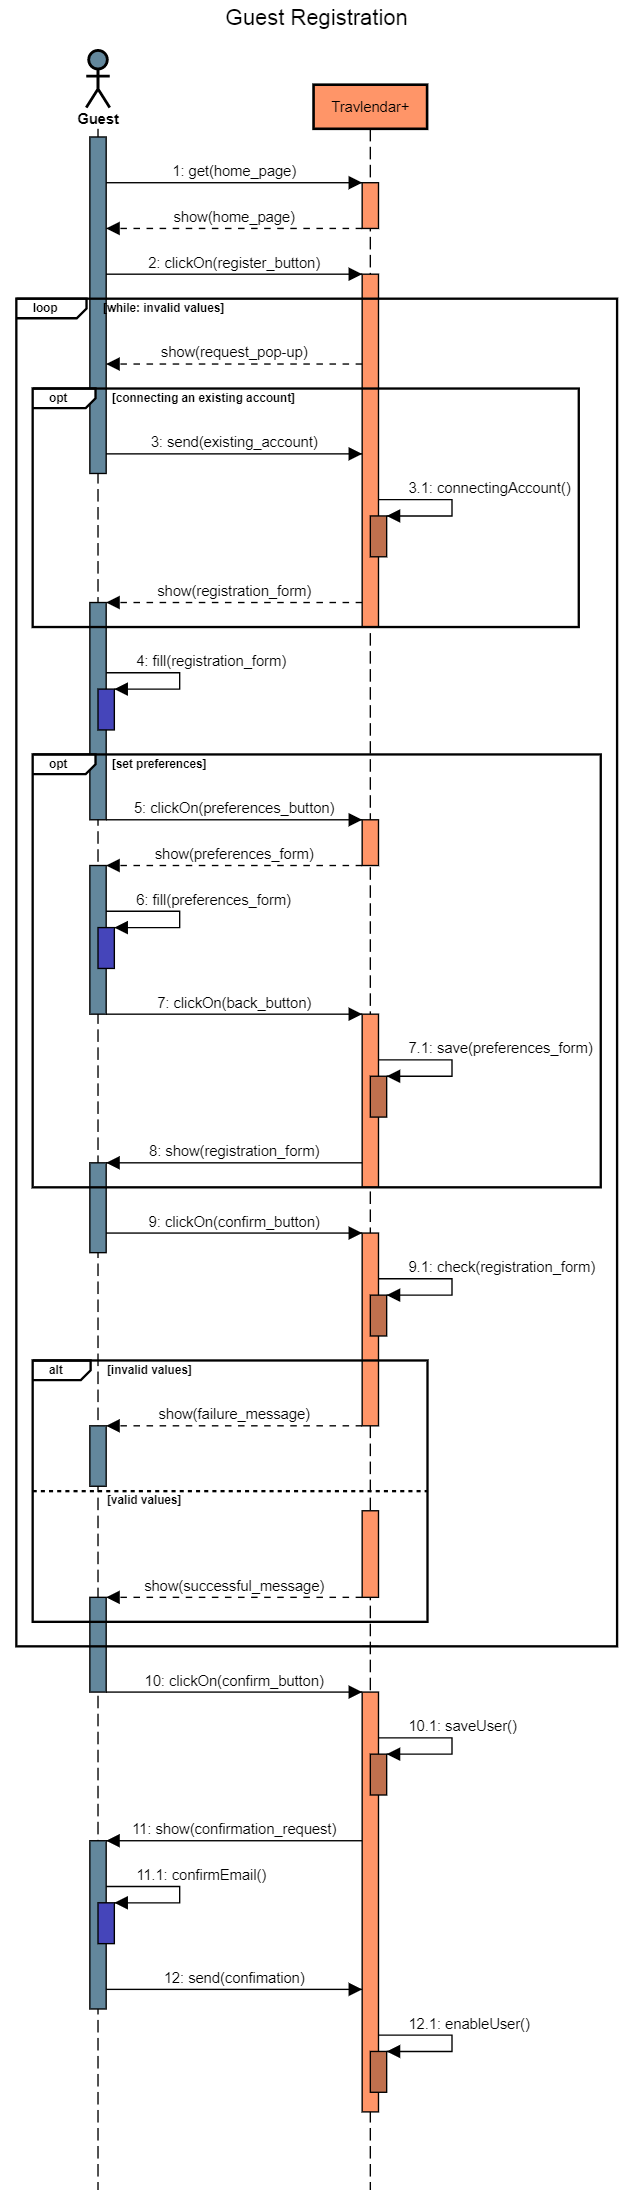
\includegraphics[width=0.50\textwidth]{Images/SequenceDiagram/GuestRegistration.png}}%
	\end{minipage}
\end{figure}
\clearpage

\subsubsection{User Login}
\begin{figure}[!h]
	\centering
	\begin{minipage}[b]{0.75\textwidth}
		\makebox[\textwidth][c]{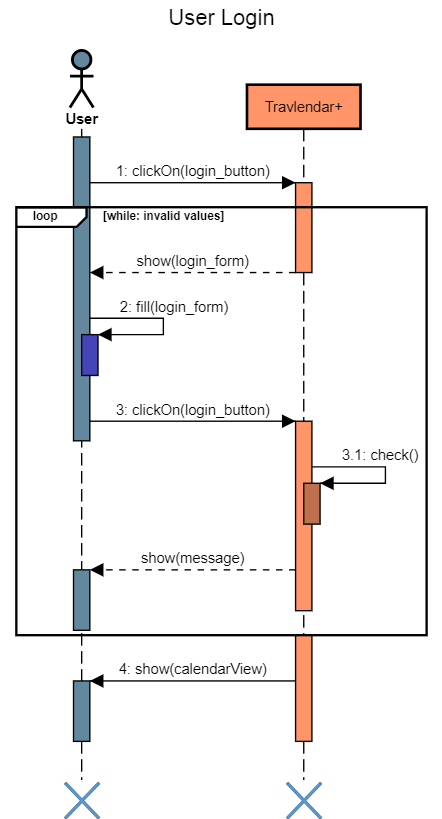
\includegraphics[width=0.50\textwidth]{Images/SequenceDiagram/UserLogin.png}}%
	\end{minipage}
\end{figure}
\clearpage

\subsubsection{Appointment creation}
\begin{figure}[!h]
	\centering
	\begin{minipage}[b]{0.65\textwidth}
		\makebox[\textwidth][c]{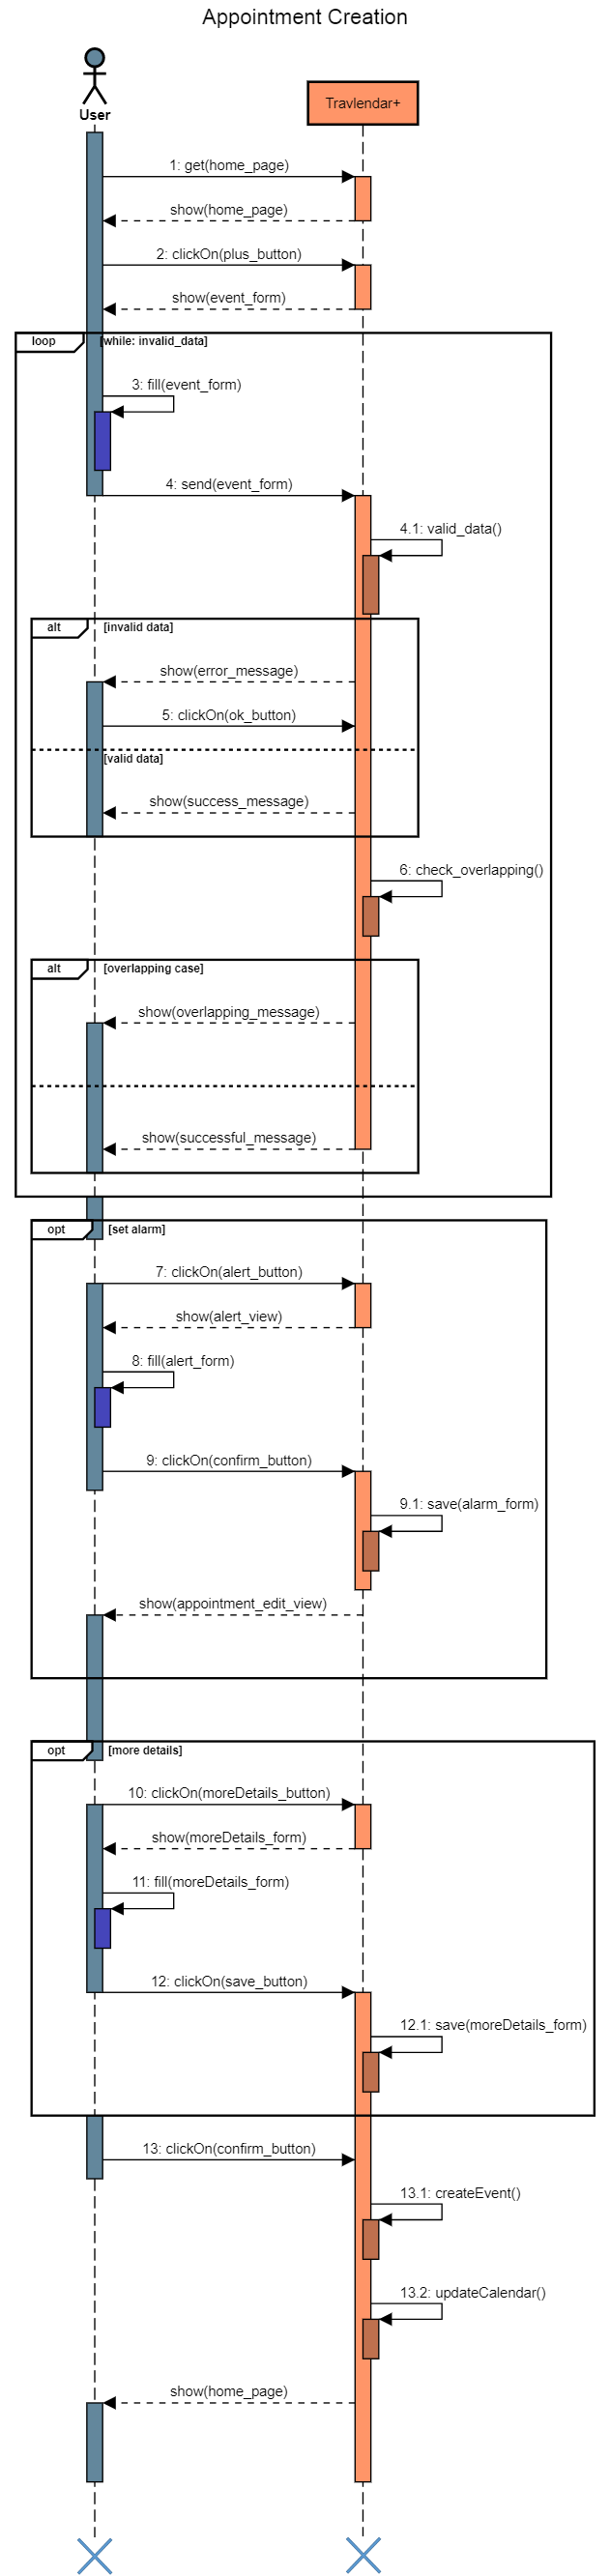
\includegraphics[width=0.50\textwidth]{Images/SequenceDiagram/AppointmentCreation.png}}%
	\end{minipage}
\end{figure}
\clearpage

\subsubsection{Appointment editing}
\begin{figure}[!h]
	\centering
	\begin{minipage}[b]{0.75\textwidth}
		\makebox[\textwidth][c]{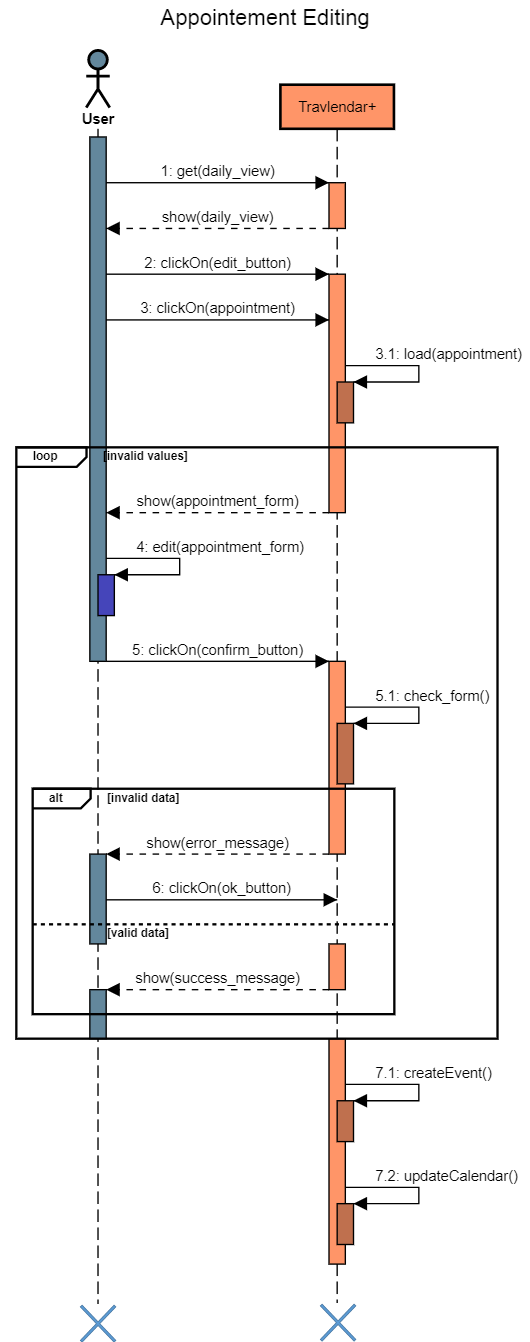
\includegraphics[width=0.50\textwidth]{Images/SequenceDiagram/AppointementEditing.png}}%
	\end{minipage}
\end{figure}
\clearpage

\subsubsection{Appointment deletion}
\begin{figure}[!h]
	\centering
	\begin{minipage}[b]{0.75\textwidth}
		\makebox[\textwidth][c]{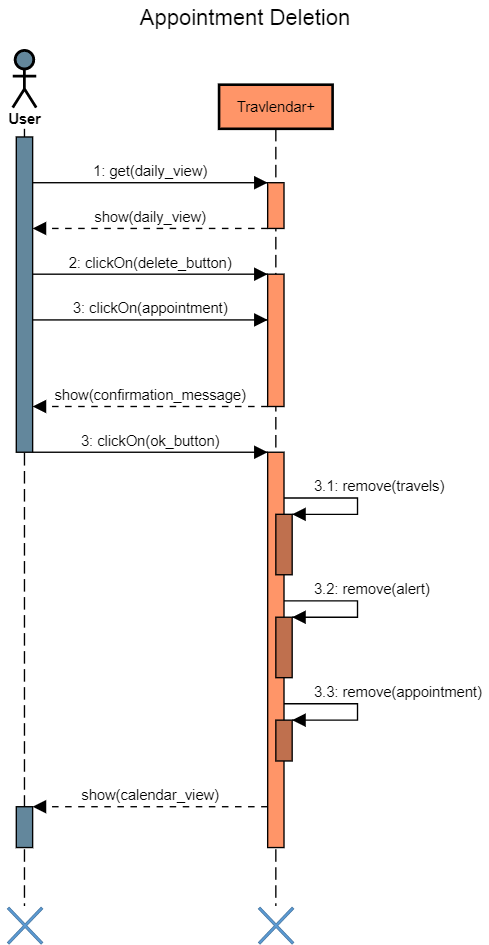
\includegraphics[width=0.50\textwidth]{Images/SequenceDiagram/AppointmentDeletion.png}}%
	\end{minipage}
\end{figure}
\clearpage

\subsubsection{Alert editing}
\begin{figure}[!h]
	\centering
	\begin{minipage}[b]{0.75\textwidth}
		\makebox[\textwidth][c]{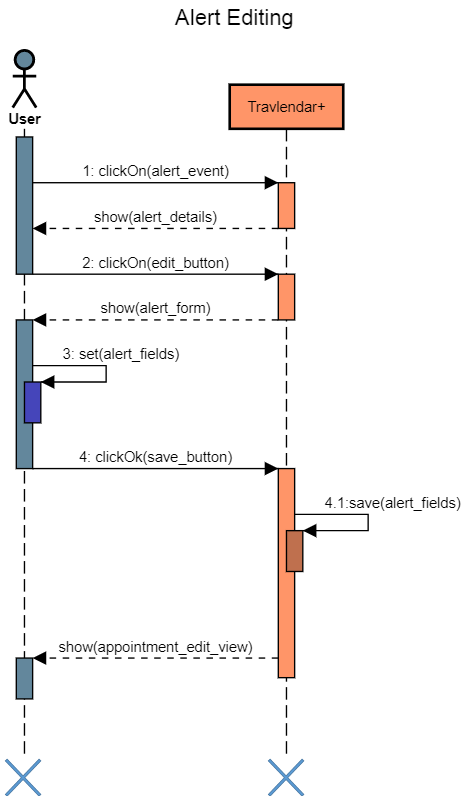
\includegraphics[width=0.50\textwidth]{Images/SequenceDiagram/AlertEditing.png}}%
	\end{minipage}
\end{figure}
\clearpage

\subsubsection{Alert deletion}
\begin{figure}[!h]
	\centering
	\begin{minipage}[b]{0.75\textwidth}
		\makebox[\textwidth][c]{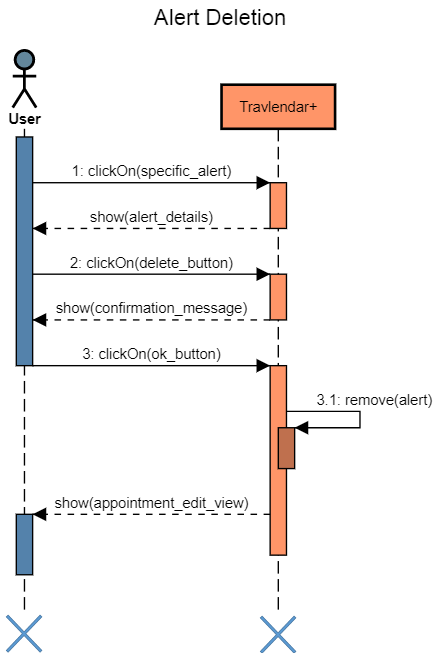
\includegraphics[width=0.50\textwidth]{Images/SequenceDiagram/AlertDeletion.png}}%
	\end{minipage}
\end{figure}
\clearpage

\subsubsection{Scheduling and view travels}
\begin{figure}[!h]
	\centering
	\begin{minipage}[b]{0.75\textwidth}
		\makebox[\textwidth][c]{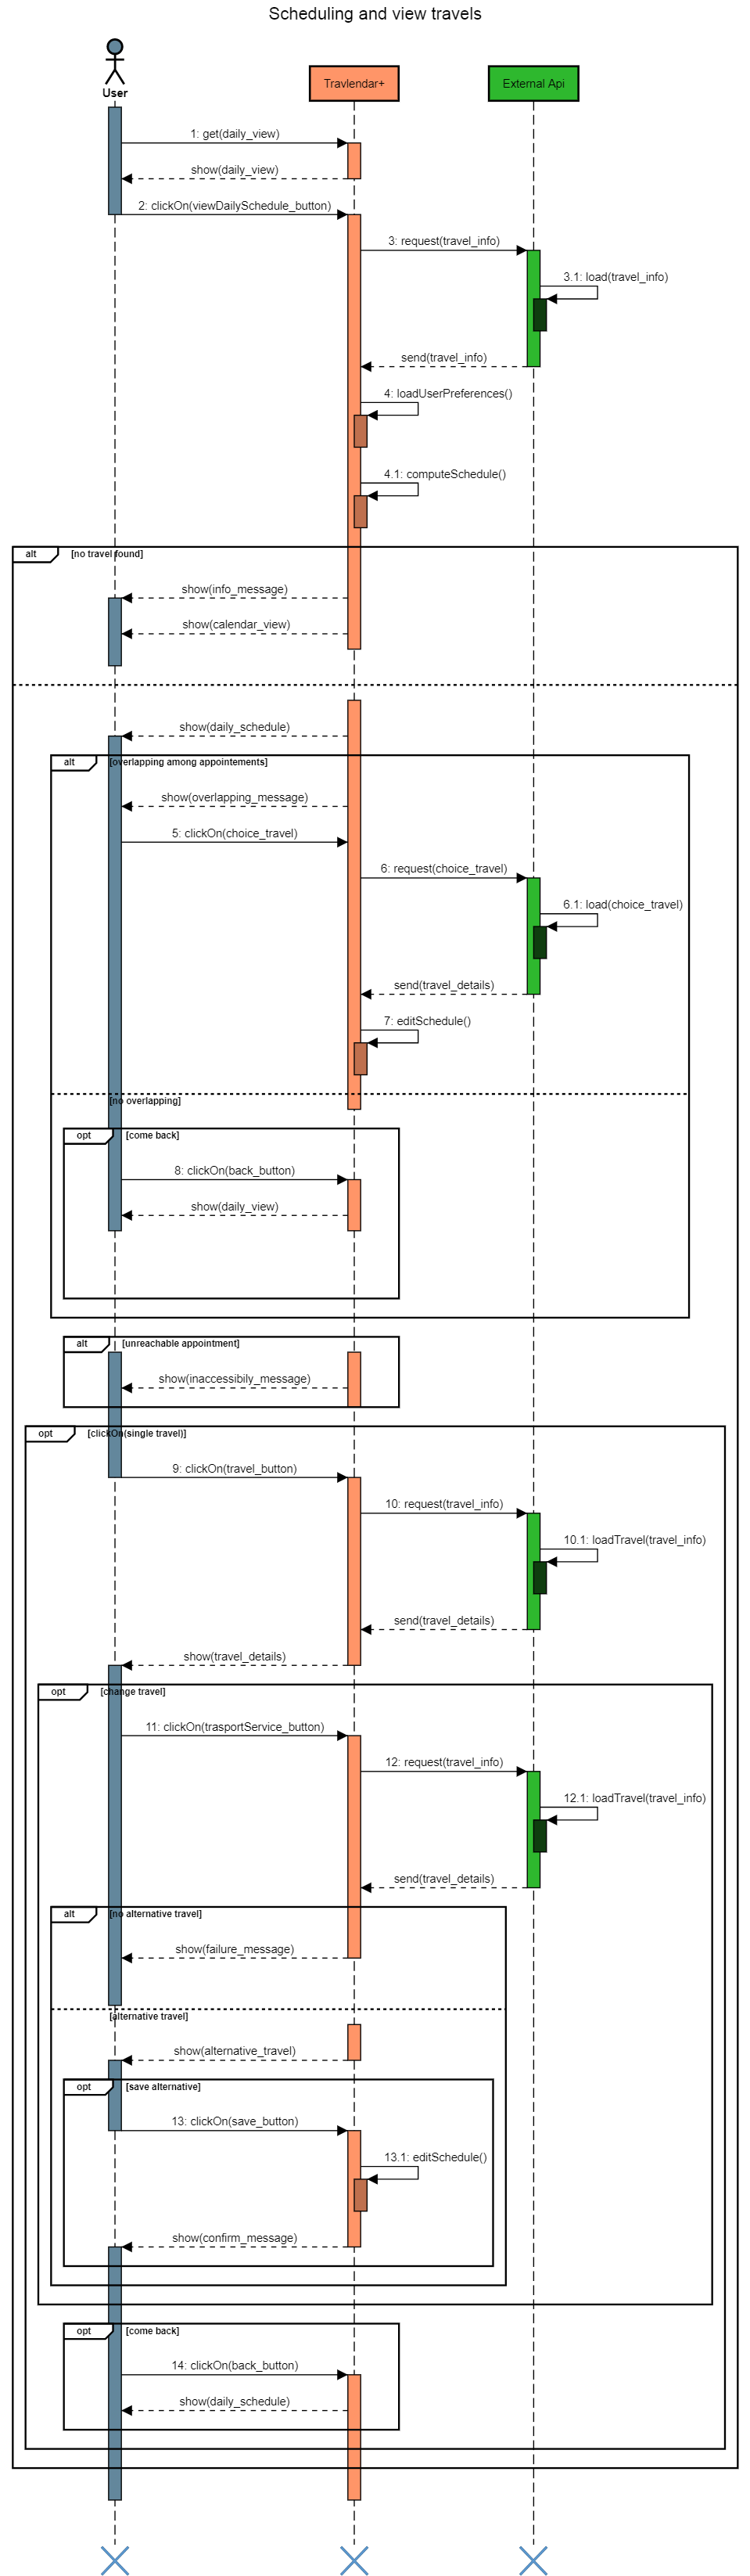
\includegraphics[width=0.50\textwidth]{Images/SequenceDiagram/SchedulingAndViewTravels.png}}%
	\end{minipage}
\end{figure}
\clearpage

\subsubsection{View and edit movements}
\begin{figure}[!h]
	\centering
	\begin{minipage}[b]{0.75\textwidth}
		\makebox[\textwidth][c]{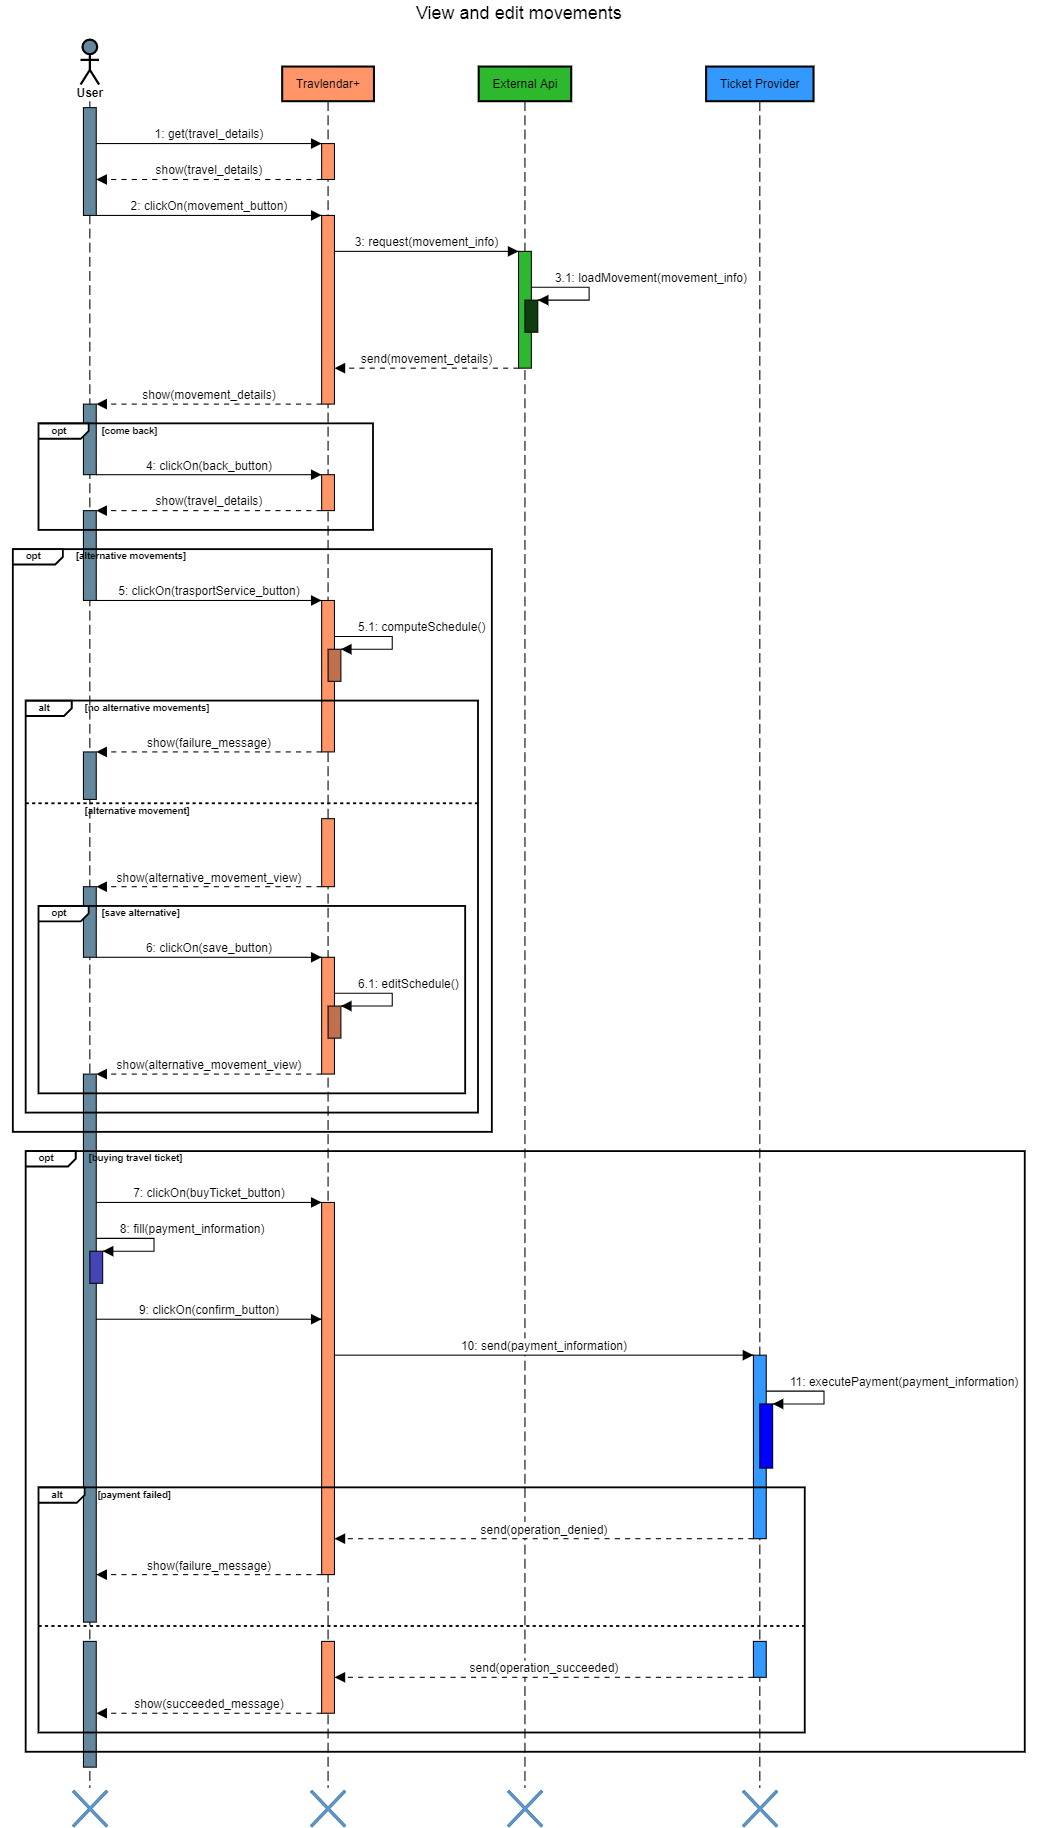
\includegraphics[width=0.50\textwidth]{Images/SequenceDiagram/ViewAndEditMovements.png}}%
	\end{minipage}
\end{figure}
\clearpage

\subsection{Activity diagram}
\subsubsection{Create appointment}
\begin{figure}[!h]
	\centering
	\begin{minipage}[b]{1\textwidth}
		\makebox[\textwidth][c]{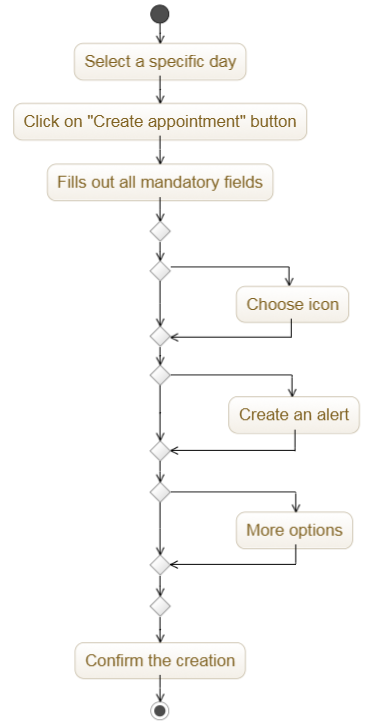
\includegraphics[width=0.50\textwidth]{Images/ActivityDiagram/CreateAppointment.png}}%
	\end{minipage}
\end{figure}
\clearpage

\subsubsection{Edit appointment}
\begin{figure}[!h]
	\centering
	\begin{minipage}[b]{1\textwidth}
		\makebox[\textwidth][c]{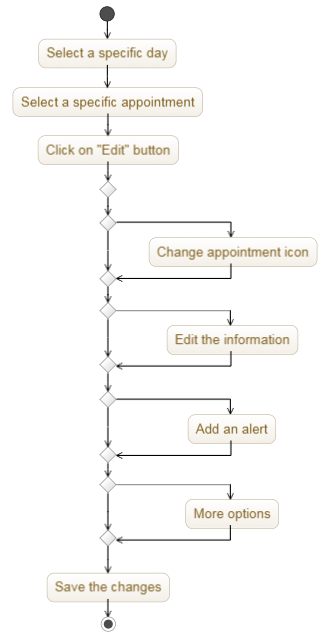
\includegraphics[width=0.50\textwidth]{Images/ActivityDiagram/EditEvent.png}}%
	\end{minipage}
\end{figure}
\clearpage

\subsubsection{Delete appointment}
\begin{figure}[!h]
	\centering
	\begin{minipage}[b]{0.8\textwidth}
		\makebox[\textwidth][c]{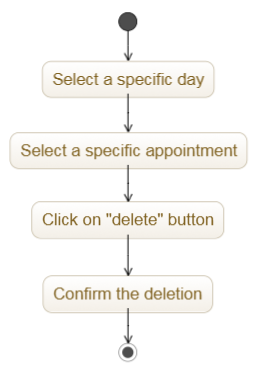
\includegraphics[width=0.50\textwidth]{Images/ActivityDiagram/DeleteEvent.png}}%
	\end{minipage}
\end{figure}

\subsubsection{Create alert}
\begin{figure}[!h]
	\centering
	\begin{minipage}[b]{1\textwidth}
		\makebox[\textwidth][c]{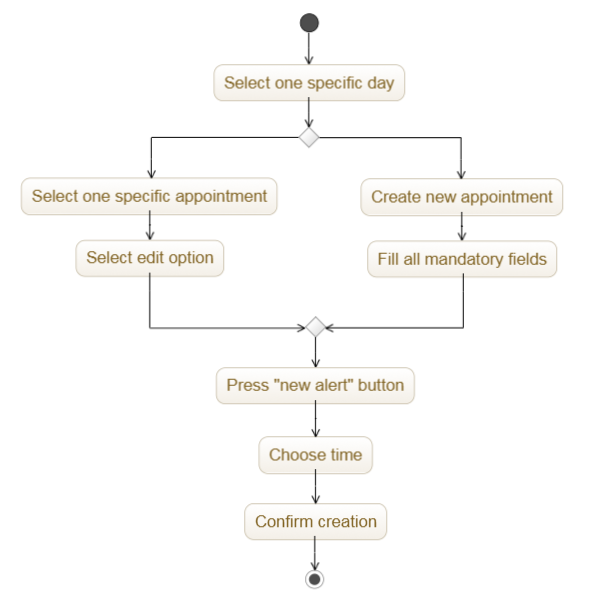
\includegraphics[width=0.50\textwidth]{Images/ActivityDiagram/CreateAlert.png}}%
	\end{minipage}
\end{figure}
\clearpage

\subsubsection{Edit travel}
\begin{figure}[!h]
	\centering
	\begin{minipage}[b]{1\textwidth}
		\makebox[\textwidth][c]{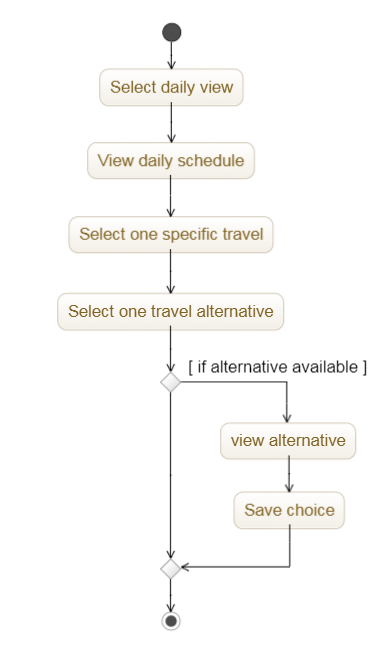
\includegraphics[width=1\textwidth]{Images/ActivityDiagram/EditTravel.png}}%
	\end{minipage}
\end{figure}
\clearpage

\subsubsection{Buy ticket}
\begin{figure}[!h]
	\centering
	\begin{minipage}[b]{1\textwidth}
		\makebox[\textwidth][c]{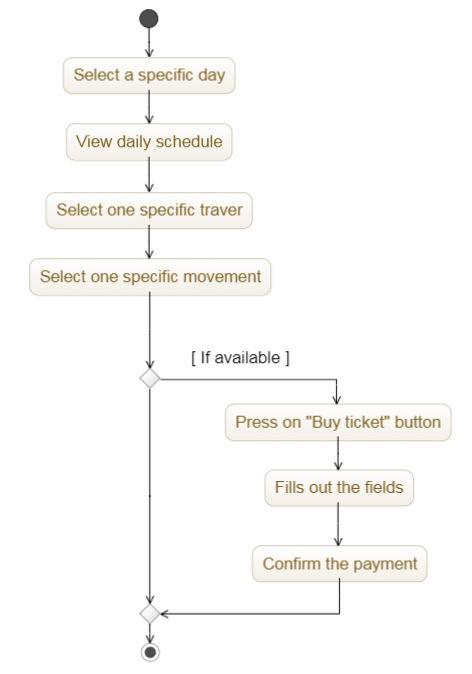
\includegraphics[width=0.50\textwidth]{Images/ActivityDiagram/BuyTicket.png}}%
	\end{minipage}
\end{figure}
\clearpage

	
	%------------------------------------------------------------------------------------------------------------------------------------------------
	\clearpage
	{\color{Blue}{\section{Formal Analysis Using Alloy}}}
	\label{sect:alloy}
	Organize this section according to the rules defined in the project description. 

	
	%------------------------------------------------------------------------------------------------------------------------------------------------
	\clearpage
	{\color{Blue}{\section{Effort Spent}}}
	\label{sect:effort}
	\subsection{Hours of work}
\subsubsection{Andrea Mafessoni}

\begin{table}[h!]
	\begin{tabular}{lcccc}
		\toprule
		\textbf{Task name} & \textbf{Start date} & \textbf{End date} & \textbf{Hours(h)} & \textbf{Day} \\
		\midrule
		\textbf{RASD} & \textbf{02/10/2017} & \textbf{28/10/2017} & \textbf{34.5} &  \\
		Thinking about project ideas & 02/10/2017 & 10/10/2017 & 5 & 9 \\
		3. Specific Requirements (Functional requirements) & 05/10/2017 & 10/10/2017 & 5 & 6 \\
		4. Scenarios & 11/10/2017 & 14/10/2017 & 3.5 & 4 \\
		5.1 Uml modelling (Use case) & 08/10/2017 & 20/10/2017 & 4 & 13 \\
		5.1 Uml modelling (Class diagram) & 10/10/2017 & 20/10/2017 & 5 & 11 \\
		6. Alloy & 14/10/2017 & 22/10/2017 & 7 & 9 \\
		\bottomrule
		Final revision & 25/10/2017 & 28/10/2017 & 5 & 9 \\
	\end{tabular}
\end{table}

\subsubsection{Andrea Mazzeo}

\begin{table}[h!]
	\begin{tabular}{lcccc}
		\toprule
		\textbf{Task name} & \textbf{Start date} & \textbf{End date} & \textbf{Hours(h)} & \textbf{Day} \\
		\midrule
		\textbf{RASD} & \textbf{02/10/2017} & \textbf{28/10/2017} & \textbf{35} &  \\
		Thinking about project ideas & 02/10/2017 & 10/10/2017 & 5 & 9 \\
		1. Introduction & 04/10/2017 & 5/10/2017 & 2.5 & 1 \\
		3. Specific Requirements (User Interface) & 06/10/2017 & 15/10/2017 & 10 & 10 \\
		3. Specific Requirements (Functional requirements) & 07/10/2017 & 08/10/2017 & 2.5 & 2 \\
		3.4 Software system attributes & 14/10/2017 & 14/10/2017 & 1 & 1 \\
		5.3 Activity diagram & 20/10/2017 & 22/10/2017 & 2 & 3 \\
		5.1 Uml modelling (Use case) & 10/10/2017 & 10/10/2017 & 2 & 1 \\
		Latex & 23/10/2017 & 28/10/2017 & 5 & 6 \\
		\bottomrule
		Final revision & 25/10/2017 & 28/10/2017 & 5 & 9 \\
	\end{tabular}
\end{table}

\subsubsection{Daniele Moltisanti}
\begin{table}[h!]
	\begin{tabular}{lcccc}
		\toprule
		\textbf{Task name} & \textbf{Start date} & \textbf{End date} & \textbf{Hours(h)} & \textbf{Day} \\
		\midrule
		\textbf{RASD} & \textbf{02/10/2017} & \textbf{28/10/2017} & \textbf{33.5} & \\
		Thinking about project ideas & 02/10/2017 & 10/10/2017 & 5 & 9 \\
		2. Overall Description & 04/10/2017 & 06/10/2017 & 2 & 2 \\
		3. Specific Requirements (Functional requirements) & 07/10/2017 & 10/10/2017 & 3.5 & 1 \\
		5.1 Uml modelling (Use case) & 08/10/2017 & 15/10/2017 & 5 & 8 \\
		5.2 Sequence diagram & 16/10/2017 & 24/10/2017 & 12 & 9 \\
		3.4 Software system attributes & 14/10/2017 & 15/10/2017 & 1 & 2 \\
		\bottomrule
		Final revision & 25/10/2017 & 28/10/2017 & 5 & 9 \\
	\end{tabular}
\end{table}
	
	
	%------------------------------------------------------------------------------------------------------------------------------------------------
	\clearpage
	\addcontentsline{toc}{section}{References}
	\bibliographystyle{plain}
	\bibliography{main}
	%------------------------------------------------------------------------------------------------------------------------------------------------
	
	
	
	
\end{document}
